\chapter{Parameters of grammaticalization}\label{chap:4}
\section{Theoretical prerequisites}\label{sec:4.1}

In the preceding chapter we saw plenty of n-tuples of syntagms whose members were said to be related to each other by grammaticalization and were therefore ordered on a grammaticalization scale. The criteria by which this was done were mentioned sporadically but not made explicit. Since different criteria were, in fact, involved, the reader may well have wondered whether a heterogeneous collection of processes were not subsumed under one heading on no theoretical grounds. In some cases I have even put syntagms on a grammaticalization scale which were not historically related. So while it is certainly time to make the criteria explicit, I should perhaps say first what is not a criterion. Namely, historical relatedness of two syntagms is not a criterion for their ordering on a grammaticalization scale. I will take up this issue in §8.3 and mention here only that grammaticalization asserts itself not only on the diachronic axis and that not all grammatical change is grammaticalization. As to the former point, different structural means synchronically present in a language may be arranged on a grammaticalization scale, e.g. the postpositions and the case suffixes of Turkish. So while the symbolism ‘x {\textgreater} y’ has been used in the meaning ‘x is grammaticalized to y’, designating, that is, a historical process, this is only a special case of the general relation ‘y is grammaticalized more strongly than x’ or simply ‘y is more grammatical than x’. As to the latter point, it has been made clear from the beginning that analogy goes hand in hand with grammaticalization and drives grammatical change just as much as grammaticalization does. So if y historically continues x, x may have been analogically changed into y. In short, historical relatedness is neither a necessary nor a sufficient condition for two syntagms to be arranged on one grammaticalization scale.

Rather than listing the criteria that have been mentioned unsystematically in \sectref{chap:3} and trying to group them systematically, I shall take here the opposite route and present them deductively. Still, the whole theory behind grammaticalization will not be expounded here, but only as much of it as is necessary to understand why these are genuine criteria of grammaticalization.

Language is an activity which consists in the creation of interpersonally available meanings, i.e. signs. This activity can be more free or more regulated; accordingly, the ways in which the signs are formed will either depend more on the actual decision of the language user or more on the social conventions laid down in the grammar. This is the most general way in which we can explain what we mean by saying that a sign may be either less or more grammaticalized, respectively.

The concept of freedom concerns the relation between the language user and the signs he uses. If we abstract from the user, we get a structural analog to this concept, viz. the \textsc{autonomy} of the sign:\footnote{This notion may go back to Meillet's seminal article, too. Cf. the quotation from \citet[131]{Meillet1912} on p. \pageref{meillet} above.} the more freedom with which a sign is used, the more autonomous it is. Therefore the autonomy of a sign is converse to its grammaticality, and grammaticalization detracts from its autonomy. Consequently, if we want to measure the degree to which a sign is grammaticalized, we will determine its degree of autonomy. This has three principal aspects. First, in order to be autonomous, a sign must have a certain \textsc{weight}, a property which renders it distinct from the members of its class and endows it with prominence in the syntagm. Second, autonomy decreases to the extent that a sign systematically contracts certain relations with other signs; the factor inherent in such relations which detracts from autonomy will be called \textsc{cohesion}. Third, a sign is the more autonomous the more \textsc{variability} it enjoys; this means a momentary mobility or shiftability with respect to other signs.

So far we have three aspects of grammaticalization, namely the decrease in weight and variability and the increase in cohesion. These are still rather abstract and difficult to operationalize as analytic criteria. There are basically two ways provided by linguistic theory in which we might make them more specific and thus more concrete. We might either relate them to the content and expression of the sign, or else to the selection and the combination of the constituents of the sign. From the operational conception assumed here it follows that the first way of subdividing the criteria will be unhelpful. The content and the expression of a sign are insolubly associated with each other. There is a far-reaching isomorphism between them which concerns not only properties of their constitution but also the quantitative aspect of their composition. There tends to be a correspondence between the size, or complexity, of the significans and that of the significatum.\footnote{See \citet{Lehmann1974}. The notion of the semantic complexity of a sign is made explicit in \citet{Lehmann1978}. The postulate of an isomorphism between significans and significatum of the language sign is an implicit cornerstone of the various conceptions of structural linguistics, especially structural semantics, and a recurrent theme in the writings of D. Bolinger. It is, however, rejected by some linguists. Thus, \citet[239]{Ronneberger-Sibold1980} is certainly not alone in claiming that the size of the significans (the “length”) of a sign is not related to the size of its significatum but is determined by the frequency of its use. These authors must be asked, first what determines the frequency of the use of a sign, and second, how those cases of isomorphism which have been empirically demonstrated are to be explained.} This isomorphism is maintained in all the linguistic operations and processes which may affect the sign; whatever may affect the content will have its consequences for the expression, and vice versa. As for linguistic operations, the homomorphism between their application to the content and their application to the expression of a sign (sometimes called “semantics” and “syntax”, respectively) is a fundamental postulate of several models of grammatical description, among them Montague Grammar. Grammaticalization belongs rather among the linguistic processes. Here, too, the various factors -- to be used as criteria of grammaticalization -- apply to the sign as a whole, they do not differentiate between content and expression. This will be seen most clearly in the parameters of variability. If their effects on content and expression can be distinguished -- which is sometimes the case with the parameters of weight and cohesion --, they affect both in a parallel fashion. This was already shown by \citet[135--139]{Meillet1912}. I will therefore not subdivide the criteria according to this dichotomy, but mention the effects of grammaticalization on the expression and the content of the sign whenever they are discernible as distinct.

On the other hand, the three main aspects of grammaticalization separate into two clearly distinct sets of criteria when they are related to the fundamental aspects of every linguistic operation, viz. the selection and the combination of linguistic signs, which I will henceforth call the \textsc{paradigmatic} and \textsc{syntagmatic aspects}. The weight of a sign, viewed paradigmatically, is its \textsc{integrity}, its substantial size, both on the semantic and phonological sides. Viewed syntagmatically, it is its \textsc{structural scope}, that is, the extent of the construction which it enters or helps to form. The cohesion of a sign with other signs in a paradigm will be called its \textsc{paradigmaticity}, that is, the degree to which it enters a paradigm, is integrated into it and dependent on it. The cohesion of a sign with other signs in a syntagm will be called its \textsc{bondedness}; this is the degree to which it depends on, or attaches to, such other signs.\footnote{\citet[8]{Bazell1949} calls cohesion what is here called bondedness.} The \textsc{paradigmatic variability} of a sign is the possibility of using other signs in its stead or of omitting it altogether. The \textsc{syntagmatic variability} of a sign is the possibility of shifting it around in its construction.

\begin{table}
\begin{tabular}{lll}
\lsptoprule
 \multirow{2}{*}{\scshape paramater} & \multicolumn{2}{c}{\scshape axis}\\ \cmidrule{2-3}
 
& \scshape paradigmatic & \scshape syntagmatic\\
 %\backslashbox[40mm]{\textsc{parameter}}{\textsc{axis}} & \scshape paradigmatic & \scshape syntagmatic\\
\midrule
\scshape weight & integrity & structural scope\\
\scshape cohesion & paradigmaticity & bondedness\\
\scshape variability & paradigmatic variability & syntagmatic variability\\
\lspbottomrule
\end{tabular}
\caption{The parameters of grammaticalization}\label{T4}
\end{table}

\newpage
These six criteria (varying subsets of which crop up sporadically in the literature\footnote{\citet[169]{Weinreich1963} uses them to make a principled distinction between lexical and grammatical meaning. \citet[Ch. I]{VanRoey1974} uses them to distinguish classes of prenominal modifiers.}) are displayed, for ease of reference, in \tabref{T4}. It should be kept in mind that some of these parameters correlate positively, others negatively. As grammaticalization increases, the parameters of cohesion increase as well, while the parameters of weight and variability decrease. This is of no theoretical significance, but merely a consequence of the choice of terms.

Furthermore, it will be seen that while grammaticalization is a process, the six parameters are not processes but properties of signs, though variable properties. Strictly speaking, what these parameters jointly identify is not the grammaticalization but the autonomy or, conversely, the grammaticality of a sign, that is, the degree to which it is grammaticalized (see p.~\pageref{page11}f). \chk%8
However, mere variation of one of these properties, namely an increase or decrease in the extent to which a sign has that property, turns it into a process which affects that sign. Thus we may say that grammaticalization as a process consists in a correlative increase or decrease -- as the case may be -- of all the six parameters taken together. See also \tabref{T6}, p. \pageref{T6}.

I have been and will be calling these six aspects of grammaticalization variously its parameters, factors or criteria. The term ``factor'' emphasizes that grammaticalization is a complex phenomenon which is constituted by these aspects and has no existence independently of them; grammaticalization is made up of these six parts. The terms ``parameter'' and ``criterion'' focus on the methodological aspects of the problem. The above six properties of linguistic signs are criteria insofar as they can be used to order two functionally similar syntagms on a grammaticalization scale. They are parameters insofar as grammaticalization may be measured along each of them, and it may then be verified to which degree they correlate.

Insofar as the six grammaticalization parameters have a common deductive basis, they are theoretically dependent on each other. However, the theoretical basis has not been made fully explicit, nor can it be, at least in this study. There are therefore no theoretical grounds on which to expect a 100\% correlation between them. The only thing that we can safely assume is that they will correlate to a significant degree. On the other hand, each of the parameters can be examined independently of the others: they are methodically independent of each other. From this viewpoint, the question of whether and to which degree they correlate can legitimately be considered an empirical question. And if they correlate, their correlation may be considered explained by the theory. Naturally, independent application of the parameters to the analysis of natural language syntagms presupposes that they are made explicit to the degree of becoming quantifiable. I will return to this problem in \sectref{sec:4.4}.

\label{page135}The comparison of two signs with respect to their degree of grammaticality presupposes that they are functionally similar. This is not a formal condition. Theoretically, if all the parameters were made fully explicit and quantifiable, we might compare any two signs at all with respect to their grammaticality, for instance the perfect tense in Latin and the genitive case in Turkish. Obviously, such a comparison would not make sense. Consider the analogous situation in markedness theory: we may well ask whether /s/ or /f/ is more marked in English, but it seems unreasonable to compare /s/ and the progressive aspect as to markedness. The requirement of \textsc{functional similarity} thus boils down to the general presupposition of any comparison that two things compared with each other should have something in common. As a methodological prerequisite, the notion of functional similarity will be taken for granted here. The only thing we have to do is to specify what kind of functional similarity we mean. Obviously, the Latin perfect und pluperfect tenses, the Hungarian allative and ablative cases or the English definite and indefinite articles may be said to be functionally similar. But these cannot be ordered against each other on a grammaticalization scale, so that this notion of functional similarity must be excluded. We do not mean that there is a common basis on top of which there may be varying and contrasting differentiae specificae. Instead, what we find in a grammaticalization channel is a function common to all the elements in it, the differences among them being primarily of a quantative nature. This is to say, two adjacent elements on a grammaticalization scale fulfill the same function, but to different degrees. For example, a demonstrative and a definite article both have the function to determine, but the demonstrative determines more specifically than the article. However, the quantitative differences between adjacent items sum up when the distances on a scale become greater, and there must certainly come a point where quantity changes to quality. For example, although a demonstrative pronoun may, in the long run, be grammaticalized into an affixal noun marker (sign of nominality), we would probably not want to say that the difference between these two signs is merely of a quantitative nature. Nevertheless, they still have a common functional basis, which is, so to speak, laid bare in the most grammaticalized member of a scale (e.g. the noun marker), but superposed by more specific functional aspects in the less grammaticalized members (e.g. the demonstrative). In this sense, the functional similarity among the elements of a grammaticalization scale is represented by its last member, something close to their common ``Gesmamtbedeutung'', the smallest common denominator to which the input of the scale reduces in the end.\label{page135b}

In what follows, we will discuss each of the six parameters in turn, highlighting its specific aspects and marking it off against other linguistic processes which are similar in appearance and may interact with grammaticalization, but must be kept distinct from it.

\section{Paradigmatic parameters}
\subsection{Integrity} \label{sec:4.2.1}

The paradigmatic weight or integrity of a sign is its possession of a certain substance which allows it to maintain its identity, its distinctness from other signs, and grants it a certain prominence in contrast to other signs in the syntagm. It is this factor of grammaticalization in which semantic and phonological aspects can be most clearly distinguished. Decrease in the semantic integrity of a sign is desemanticization; decrease in the phonological integrity is phonological attrition. The parallelism between these two processes has been emphasized repeatedly in the literature; see \citet[135--139]{Meillet1912} and \citet[114--119]{Lehmann1974}. I will subdivide the discussion accordingly.

%\setcounter{page}{1}
\textsc{phonological attrition} (called erosion in \citealt[21ff]{HeineEtAl1984} and decay elsewhere) is the gradual loss of phonological substance. We may assume here that the significans of a sign is represented as a two-dimensional matrix of marked phonological features. A column in the matrix is a segment, and it must contain at least one such feature. Now attrition may be described as the successive subtraction of phonological features. Depending on where features are subtracted, this may also lead to the loss of segments; then the result is, of course, that the sign becomes shorter. With the loss of the last feature, the whole significans disappears. Since phonological attrition and desemanticization go hand in hand, this accident normally means that the significatum is also lost, so that the sign ceases to exist. However, this is not always so, as we shall see later on. Anyway, this is perhaps the factor which can most straightforwardly be operationalized, since little more than counting of phonological features is involved.

Examples of phonological attrition picked at random from \sectref{chap:3} are the reduction of Latin \textit{ille} to French \textit{le} (frequently /l/), Proto-Indo-European *\textit{esti} {\textgreater} Engl. \textit{is} (frequently /z/), PIE *\textit{oinos} {\textgreater} Engl. \textit{a} (i.e. /ə/). \citet[25]{HeineEtAl1984} have an impressive example from Duala (Bantu): Proto-Bantu *\textit{gide}, probably some verb meaning ‘finish’, {\textgreater} -\textit{gide} \glcompl {\textgreater} -\textit{ide} {\textgreater} \textit{í} {\textgreater} \textit{\'{ }} (i.e. high tone). The example shows that phonological attrition may indeed leave exactly one phonological feature of an erstwhile multisegmental significans.

It is obvious that phonological attrition is omnipresent in linguistic change. It plays its role not only in grammaticalization, but affects, in the long run, practically every sign. Examples outside grammaticalization are the reduction of Latin \textit{aqua} ‘water’ to French \textit{eau} (i.e. /o/) or of PIE *\textit{k}\textit{\textsuperscript{w}}\textit{etwores} to Engl. \textit{four} (i.e. /fɔ:/). Consequently, it would be wrong to infer from phonological attrition to gramamticalization. We will meet the same situation with some of the other parameters. None of them is by itself sufficient to define grammaticalization; it is only by the interplay of all of them that grammaticalization comes about.

We may preliminarily raise here the question of the causal relationships between phonological attrition and anything else. On the one hand, some linguists believe that virtually all of linguistic change is a consequence of the reductive phonological evolution. The latter leads to the loss of inflection and therefore to grammatical renovation or even innovation, and it leads to the loss of lexical items and therefore to constant neology. Phonological attrition itself, in this conception, is essentially a consequence of the articulatory inertia of the speaker who follows the principle of least effort. Other linguists think rather that phonological attrition is merely a symptom of functional changes going on in the system, that inflectional morphology gets lost not on phonological, but on semantosyntactic grounds. I should prefer to treat this -- certainly complex -- problem not in such an isolated fashion, but to gather insights on the behavior of each of the parameters and then try to obtain an integrated picture of eventual causal or hierarchical relationships among them. In the other parameters to be discussed, I will therefore not devote special attention to questions of this sort.

We now turn to the semantic integrity or \textsc{semanticity} of a word. For the sake of simplicity, I will assume that the semantic representation of a sign consists of a set of propositions taken from some semantic metalanguage commonly called semantic components or features, and that those propositions which are conjoined (rather than disjoined) contribute to the semantic complexity or semanticity of the sign (details in \citealt{Lehmann1978}). \textsc{Desemanticization}, or semantic depletion \citep[180f]{Weinreich1963} or bleaching, is then the decrease in semanticity by the loss of such propositions. As said above, the last proposition is commonly lost at the moment where the last rest of the significans also disappears; but as we shall see, either one can continue, at a submorphemic level, without the other. The operationalization of this criterion is in principle completely parallel to that of phonological attrition, except that semantic representations of the required sort are not always easy to come by.

Here are some examples of desemanticization: Latin \textit{d\=e} ‘down from (the top)’ (cf. pp.~\pageref{page78b}--\pageref{page79}\chk%65
) had a delative meaning. That is, in x \textit{de} y, x is on top of y at some prior time, but then moves down and away from y. In the Romance development, what got lost first was the first, specifically delative component, and what remained was the ablative meaning ‘from’. (This is, by the way, an example of a possible leftward prolongation of the scale in \figref{F8}, p. \pageref{F8}). On its way towards French \textit{de} (note the phonological attrition from /d\=e/ to /d/), the motion component was lost, too, so that the ablative was reduced to the genitive ‘of’, the sheer notion of a relation between two entities. OE \textit{sceal} ‘owe’ specifies that what the subject has to do is to pay an amount of money or otherwise to return something to somebody. First this specification is lost, and only the meaning that the subject has to do something is left. Then the deontic component is lost, too, and what remains is an indication that the subject will do something. Finally, Latin \textit{h\=ac h\=or\=a} ‘at this hour’ was grammaticalized to Port. \textit{agora}, Spanish \textit{ahora} ‘now’. Here the generic temporal component and the deictic element pointing to the time of the speaker go through to the end, but the specification of the time unit present in the source is lost underway.

Just as phonological attrition, desemanticization occurs outside grammaticalization as well. I will defer discussion of this phenomenon to §.~5.1 and dwell here on the manifold aspects of desemanticization within grammaticalization. The principal interest of scholars since W. \citet[52]{Humboldt1822} has centered around “die Stufenfolge, in welcher die ursprüngliche Bedeutung sich verloren hat”.  There are descriptive terms available for the kind of semantic variation to be found in a grammaticalized item: at the source of a grammaticalization process, we have the ``Grundbedeutung'' (core meaning) of the item; at the end, we have its ``Gesamtbedeutung'' (general meaning; cf. \citealt{Jakobson1936}). This relationship manifests itself both diachronically, as the semantic gradation that Humboldt had in mind, and synchronically, as a specific kind of polysemy. It is illustrated with particular clarity by \figref{ex:F6} on the grammaticalization of coverbs and \figref{F8} on the grammaticalization of cases. The literature contains a wealth of proposals to account for this kind of ordered semantic variation. Two of them will be selected for review here (see, in additon, \citealt{Traugott1980}).

The most conservative conception was first formulated by E. \citet[Ch.~V]{Sapir1921} and has already been shown (p. \pageref{SapirHumCh4}) to continue certain ideas of Humboldt's. Sapir sets up four classes of concepts (displayed on p. \pageref{SapirHumCh4} above) which run the gamut from the most concrete to the most abstract or, according to his conception, from “material content” to “pure relation”. He gives no criteria by which a meaning can be assigned a place between these two poles. His proposal has, nevertheless, appeared attractive to more recent authors and is taken up by \citet[83]{Žirmunskij1966} with the words:

\begin{quotation}
The grammaticalization of the word combination is connected with a\linebreak greater or lesser weakening of the lexical meaning of one of its components, its consistent transformation from a lexically meaningful (presentational) word into a semi-relational or relational word ... The grammaticalization presents the result of the abstraction (sometimes more, sometimes less full) of the concrete lexical meaning which the function word initially had.
\end{quotation}

\noindent Here we meet the same pairs ‘concrete/abstract’ and ‘presentational/relational’. It appears that while the first opposition is correct, the second has nothing to do with grammaticalization. Since the initial meaning is richer, more specific, it is also more palpable, more accessible to the imagination (“anschaulich”) and, in this sense, more concrete; whereas the meanings of strongly grammaticalized signs, such as ‘of’, ‘will’ or ‘and’, do not yield mental images, cannot be illustrated and are, in this sense, more abstract. On the other hand, if ``relational'' is not just another word for ``grammatical'', but has its technical meaning of ‘embodying a relation, i.e. having an open slot for an argument’, then it seems clear that relationality is not affected by grammaticalization. More specifically, in the most straightforward cases relational lexemes yield relational grammatical formatives, and absolute lexemes yield absolute grammatical formatives. Cross-overs may occur, but are not part of the grammaticalization process (cf. \pageref{page73}\chk%60
). Typical examples include: Latin \textit{de} {\textgreater} French \textit{de}, both relational; Pre-Latin *\textit{ne-hilum} ‘not a thread’ {\textgreater} Lat. \textit{nihil} ‘nothing’, both absolute; Latin \textit{ille} {\textgreater} French \textit{le}, both relational, if determiners, both absolute (or only anaphorically relational), if pronouns; etc.

One point, however, may be conceded: The relationality (or absoluteness) of an item is part of its grammatical features. Grammaticalization rips off the lexical features until only the grammatical features are left.\footnote{This is a major theme in \citet{Givón1973}.} Consequently, the relationality of an item is normally conserved while most of the original semantic features are lost in grammaticalization. Therefore, it is frequently the case that the end-product of the process signifies little more than a kind of grammatical relation. French \textit{de} is again an example.

The second proposal which has some adherents today can be traced back to H. \citet[233]{Frei1929}:

\begin{quote}
Examiné du point de vue le l'évolution, le langage présente un passage incessant du signe expressif au signe arbitraire. C'est ce qu'on pourrait appeler la loi de l'usure: plus le signe est employé fréquemment, plus les impressions qui se rattachent à sa forme et à sa signification s'émoussent. Du point de vue statique et fonctionnel, cette évolution est contre-balancée par un passage en sens inverse: plus le signe s'use, plus le besoin d'expressivité cherche à le renouveler, sémantiquement et formellement.
\end{quote}

\noindent This passage has been quoted here in full because it contains a whole grammaticalization theory in a nutshell. We shall return to other aspects of it later on and concentrate here on the opposition ‘expressive/arbitrary’. It implies the equivalence ‘expressive = non-arbitrary = motivated’. This conception apparently relies on the fact that at the beginning of a grammaticalization scale we have periphrastic or even textually free constructions whose constructional meaning is motivated either by the syntax or even by functional sentence perspective. These are more expressive in the sense in which more transparent, more sumptuous constructions are more expressive than opaque or reduced ones. Compare, for example, the use of cleft-sentences with that of focus particles in focussation, the appositive juxtaposition of an anaphoric attribute to the use of a plain attribute in attribution%
%Beispiel geben
, or the use of a relational noun and that of a simple adposition (e.g. \textit{in} \textit{back of} vs. \textit{behind}) in adverbial relations. The same opposition is even valid for the single lexeme vs. grammatical formative. To signify \textsc{dative} with the help of a coverb with the basic meaning ‘give’ is palpably more expressive than to use a mere \textit{to} or even a case suffix for this purpose, because it makes the formation of a mental image for a grammatical concept possible; whereas Engl. \textit{to} evokes no associations, might as well be called otherwise and is, in this sense, arbitrary. Indefinite pronouns and negations are further examples of categories which lose their initial emphasis in the course of grammaticalization.

\label{page140}This concept of \textsc{demotivation} (cf. the quotation from Hagège on p. \pageref{Hagege} above) has been extended by recent writers, with farreaching consequences. \citet[208--233]{Givón1979b} opposes, within the left half of a grammaticalization scale (\figref{fig:phases}), the “pragmatic mode” to the “syntactic mode”, characterizing the pragmatic mode as more transparent.\label{page141b} \citet[170--172]{Vincent1980a} equates ‘weakly grammaticalized = pragmatically motivated = iconic’ and ‘strongly grammaticalized = unmotivated = arbitrary’. Finally, \citet[622]{Plank1979b} opposes “functionally based coding” to “grammaticalized, functionally invariable language-particular coding”, where the former observes only universal requirements of semantic distinctness, while the latter is largely arbitrary. Plank's equation ‘pragmatically/functionally motivated = universal’ and ‘arbitrary = language-particular’ can also be found in the two other sources quoted. I will defer a fuller discussion of the problems involved here until §§6.4 and 7.3.\label{page141}

We may anticipate that there is doubtless a grain of truth in these suggestions; but it is easy to overstate the case. There is an inveterate preconception in much of the linguistic literature which may be expressed by the equation ‘grammaticalized = unmotivated = non-functional (or even dysfunctional)’. The reasoning behind this is, of course: if something is desemanticized, it ends up having no meaning; if it has no meaning, it contributes nothing to the message and is, therefore, functionless. Examples that have been raised repeatedly in the literature include the category of gender as it appears, e.g., in Latin or German, the English infinitive marker \textit{to} and the \textit{do} appearing in interrogative and negative sentences (cf. \citealt[97f]{Sapir1921} , \citealt[421]{Lyons1968}). We shall see in \sectref{sec:4.2.3} that, quite on the contrary, the more grammaticalized an element gets, the more functional in its language system it becomes; and again, if something is not grammaticalized, it is not functional in its language system.

\enlargethispage{1\baselineskip}
One particular type of demotivation deserves some attention here. As is commonly known, there is, within the formal process of \textsc{reduplication}, a gamut of completeness, leading from total reduplication, as in Indonesian \textit{orang-orang} (man-man) ‘men’, via syllable reduplication, as in Hua \textit{kire'-are'} (corn-\rdp) ‘lots of corn’ \citep[222]{Haiman1980}, to segment-reduplication, as in Latin \textit{pe-pul-i} (\rdp-drive.\pf-1.\glsg) ‘I drove’. Parallel to the decrease in substantive completeness, there is an increase in phonological regularity and thus formal grammaticalization. Again in parallel, we have a decrease in the iconicity of the meaning represented by the reduplication (cf. \citealt{André1978} and \citealt[46--48]{HeineEtAl1984}). Full reduplication tends to signify intensification; for instance, with nouns, a multitude or collectivity, and with verbs, an intense or repeated action. More “domesticated” reduplication may signify grammatical meanings a bit more remote from the basis, such as plural or durativity. Arbitrary functions, such as the formation of perfect stems in ancient Indo-European languages, are presumably only found in fully phonologized reduplication.

Thus, reduplication illustrates in a particularly clear fashion what is meant by demotivation in grammaticalization. The example might appear to be problematic, though, since it differs in a crucial respect from all the other instances of grammaticalization we have considered so far. Only here, a grammaticalization channel appears to be defined by a formal process, instead of by a function, or set of functions. On closer inspection, however, the exception proves to be a matter of perspective. We have taken the onomasiological perspective throughout, starting from functionally defined grammaticalization scales and occasionally narrowing down on a grammaticalization channel as a particular diachronic-structural instantiation of a scale. In a semasiological perspective, we could set up purely structural scales, based on means of expression such as prefixation, suffixation, reduplication etc. If we took such formal means as the point of departure and sought, in an inductive and semasiological procedure, the functions associated with them, this would lead to results of varying specificity. While all the functions fulfilled by prefixation might well turn out to have nothing in common, and similarly those fulfilled by suffixation and infixation -- but this would have to be verified --, reduplication does appear to have a uniform functional basis, namely multiplication/intensification. This is doubtless a consequence of the fact that the formal process of reduplication is much more narrowly defined than the other ones, which correlates with the further fact that it is much less used in grammars than the other processes.

We should finally note that there is one aspect of the reduction of the paradigmatic weight of a sign in which the distinction between processes affecting the significans and processes affecting the significatum is not so easily made. This is the loss of the ability to inflect. This has been used as an independent criterion of grammaticalization in \citet[84]{Givón1975}; but it is an integral part of the reduction of the integrity of the sign. A clear example are coverbs; when these develop into adpositions or conjunctions, they cease to take affixes according to the verbal categories of the language. The history of the English modals is a related example.

Sometimes one inflectional subcategory becomes invariably associated with the grammaticalized lexical item and gets petrified on it (cf. p.~\pageref{page147}\chk%121
  on fossilization). For example, relational nouns on their way towards adpositions first take only a limited number of case affixes, viz. only local ones. This is the situation in Quechua (see p.~\pageref{page87}\chk%72
) and Hittite (p.~\pageref{page98}--\pageref{page100b}\chk%81
). In a second step, the choice is reduced to one case affix, and this is then welded together with the noun to yield an adposition. This is the situation of the genuine postpositions of Turkish (see p.~\pageref{page86}\chk%71
). German \textit{würde} and \textit{möchte} are auxiliaries of the subjunctive and desiderative, respectively. They only occur in finite forms of what is formally the past subjunctive and are no longer synchronically related to \textit{werden} ‘become’ and \textit{mögen} ‘may, like’.

It would be wrong to explain the loss of the ability to inflect either by phonological attrition or by desemanticization alone. Both interact to constitute what might be called \textsc{morphological degeneration}. What is lost is not some arbitrary phonological or semantic feature, but an inflectional category. The loss of all inflectional categories is the symptom of a change in status. A grammaticalized sign moves down the grammatical levels, from phrase via word form to morpheme. The last step, in particular,  involves, in the first place, its transition from a major category to a minor one. We will have to take this point up in the next section.

\subsection{Paradigmaticity} \label{sec:4.2.2}

What is meant here by paradigmatic cohesion or paradigmaticity is the formal and semantic integration both of a paradigm as a whole and of a single subcategory into the paradigm of its generic category. This requires that the members of the paradigm be linked to each other by clear-cut paradigmatic relations, especially opposition and complementarity. The most superficial and evident aspect of paradigmaticity is the sheer \textsc{size of the paradigm}. Consider the grammaticalization of local relational nouns to adpositions. In English, there is a fair number of such nouns as \textit{front}, \textit{back}, \textit{top}, \textit{bottom}, \textit{interior} etc. which may be used to form periphrastic prepositions. These are opposed to a closed but still relatively large set of secondary local prepositions such as \textit{beyond}, \textit{before}, \textit{within}, \textit{amidst} etc. Finally, we have the small set of primary local prepositions including \textit{in}, \textit{on}, \textit{at, from, to} and perhaps some others.

Similar numerical relationships may be found in the grammaticalization of -- numeral or possessive -- classifiers to noun classes and genders: the former may range in the dozens, whereas the latter are usually few, often only two. Again, consider personal pronouns (cf. \sectref{sec:3.2.1.2}). In Japanese, these are grammaticalized very little and agglomerate to a poorly integrated paradigm of at least twelve forms for the first and second persons (unmarked for number) which offer a choice among different social relationships (see \citealt{Alpatov1980} and \citealt{Coulmas1980}). English, on the other hand, possesses fully grammaticalized personal pronouns forming a tightly knit paradigm of five distinct forms. Lastly, the grammaticalization of aspect to tense is always accompanied by a reduction in the size of the paradigm. In the vast majority of languages, there are no more than three tenses, present, past and future, and often there are only two, either future and non-future (= \textsc{real}), e.g. in Dyirbal or in Turkish nominalized clauses, or past and non-past, e.g. in Walbiri. Aspect, on the other hand, can be differentiated in rich paradigms. Portuguese, for instance, has three tenses, with an analytic, slightly aspectual alternative for the synthetic future (\textit{vou} + inf. ${\simeq}$ inf.-\textit{ei}), but at least the aspectual forms shown in \tabref{T5}.

\begin{table}
\begin{tabular}{llll}
\lsptoprule

\scshape auxiliary  & &  \scshape full verb & \scshape meaning\\
\midrule
\textit{estou} & \textit{por} & + inf. & inceptive\\
\\
\textit{estou} & \textit{a} &  + inf. & \multirow{2}{*}{progressive}\\
${\simeq}$ \textit{estou} & & + ger. \\
\\
\textit{vou}/\textit{ando}  & &  + ger. & durative\\
\\
\textit{venho} & \textit{a} & + inf. & \multirow{2}{*}{resultative}\\
${\simeq}$ \textit{venho}  & &  + ger. \\
\\
\textit{acabo}/\textit{venho} & \textit{de} & + inf. & recent past\\
\\
\textit{tenho}  & & + part.pass. & perfect\\
\lspbottomrule
\end{tabular}
\caption{\textsc{tense/aspect} periphrases in Portuguese}\label{T5} 
\end{table}

\noindent The distinction between open sets of lexical items and closed sets of grammatical(ized) items is related to that between \textsc{major and minor categories} or word classes (cf. \citealt[435f]{Lyons1968}). A lexical item belongs, roughly, in one of the major classes of nouns, adjectives, numerals or verbs. The minor classes of grammatical items are, essentially, pronouns, auxiliaries (and the like), adpositions and conjunctions (particles and interjections remain unclassified). All the major classes have been shown to furnish items which enter into grammaticalization channels, and all the minor classes have been shown to be formed, or at least to receive members, through grammaticalization. For example, we have seen full verbs becoming auxiliaries, and nouns becoming numeral classifiers.

However, both the distinction between open and closed sets and the one between major and minor categories are gradual. Whether a word belongs already in the minor category of adpositions or yet in the major category of transitive verbs is a matter of degree of grammaticality. Sets are not either open or closed, but rather the fewer members they have the more closed they are. Furthermore, the distinction between major and minor categories reflects only certain segments at the beginning of a grammaticalization scale, since it presupposes words. The process, however, in which sets develop into paradigms and become ever smaller and more closed continues on the right half of a grammaticalization scale and concerns bound morphemes just as much as free morphemes.

The size of a paradigm is, to repeat it, a superficial and not always reliable aspect of paradigmaticity. Over and above its sheer size, the integration of the paradigm has more intrinsic and less easily quantifiable aspects. It also comprises the formal and functional \textsc{homogeneity} of the paradigm, i.e. a certain amount of similarity among its members and of regularity in their differences. For example, the Japanese case particles all have the canonical form (C)V, and the Turkish case suffixes have the form -(C)V(\textit{n}). Latin personal endings on the present active verb are monophonematic in the singular and bi- or triphonematic in the plural, all but one allomorph ending in a consonant. All Latin negative indefinite pronouns begin with \textit{n}. All English interrogative pronouns, with the partical exception of \textit{how}, have an expression feature in common which has enabled the denomination of the class as ‘\textit{wh-} pronouns’. \citet[256f]{Bloomfield1933} demonstrates how formally homogeneous the personal pronouns are in several unrelated languages.

On the semantic side, the members of a paradigm have a common semantic basis with varying differentiae specificae. This would be brought out by a componential analysis and is reflected in traditional terminology by the fact that there is a generic category name for the whole paradigm and oppositive names for the specific subcategories (e.g. local cases: locative, ablative, allative).

Such paradigmaticity is gradually reached in the process of grammaticalization. Categories grammaticalized very little do not constitute such tightly integrated paradigms. Consider, for example, the formal variation exhibited in the set of Portuguese aspects displayed above. Again, at the level of adpositions, many languages such as Mandarin have both pre- and postpositions, with rather heterogeneous functions (see \citealt{Hagège1975}). At the level of case markers, most languages have only suffixes. Numeral classifiers often divide up into a number of heterogeneous subclasses with different distribution and formal properties; noun classes and genders are much more homogeneous.

The process of paradigmatic integration or \textsc{paradigmaticization} leads to a levelling out of the differences with which the members were equipped originally. Genetic differences among prepositions of different origins, which account for their different behavior as long as they are weakly grammaticalized, are adjusted when they develop into primary prepositions. This can be seen, e.g., in German \textit{während} = Engl. \textit{during}, which no longer behave as participles. In German, primary prepositions govern either the dative or the accusative, but not the genitive. Secondary prepositions of nominal origin do, of course, take the genitive; but the more grammaticalized they are, the more they prefer the dative. The fate of \textit{wegen} ‘because of’ is widely known. Finally, the infinitives of ancient Greek derive from (locative) case forms (see \citealt[196f, 237--239]{Rix1976}). In historical times, however, they are well integrated into the conjugation paradigm and participate in the verbal categories of tense, aspect and voice.

In many cases of paradigmaticization, grammaticalized elements join preexistent paradigms and assimilate to their other members. The ancient Romance synthetic future, which assimilates to the suffixal tense categories is a clear case in point. Such phenomena do not result exclusively from grammaticalization; analogical levelling plays a great role in them. This does not, however, mean that paradigmaticization can be reduced to the workings of analogy. The formation of new paradigms, as, e.g., the paradigm of the definite and indefinite articles, would be impossible if it were not part of the more comprehensive grammaticalization process.

In the writing of a grammar, there is the notorious problem of whether and to what extent \textsc{periphrastic constructions} have to be admitted. Noone doubts that the synthetic verb forms and primary prepositions must be treated in a grammar; but disagreement arises when analytical verbs forms or compound prepositions are to be enumerated. The criterion that has commonly been employed by grammarians -- though with different conclusions -- is that of paradigmaticity. Thus \textit{want} does not participate in analytic verb forms since \textit{I want to write} is formed according to the same rules of syntax as \textit{I intend to write} and similar constructions with an open set of governing verbs. But \textit{will} does participate in analytic verb forms because there is a paradigm containing \textit{I will write} and a few similar constructions.%
%want solte gegen plan o.ä. ausgetauscht werden, sonst muß man Bolinger 1980 (wanna) diskutieren. Lt. Krug 1997 ist die Grammatikalisierung von wanna schon weit fortgeschritten.

The existence of a paradigm has even been made a presupposition of the correct application of the terms ``analytic'' or ``periphrastic''. Thus \citet[55]{Matthews1981} defines: “When a form in a paradigm consists of two or more words it is \textsc{periphrastic}.” This implies that if there is no paradigm, there is no periphrastic word form, but merely a combination of words (cf. \citealt[82--87]{Žirmunskij1966}). Whether or not there is a paradigm is, however, not always easy to decide or even in principle a matter of a yes-no decision. When the compound constructions are paralleled, in all relevant respects, by synthetic forms which belong to the same superparadigm, then the decision is facilitated. If such a parallelism does not obtain, as e.g. in the case of the Portuguese aspect formations, there can be only a more-or-less decision, and the question of whether such syntagms must be treated in the grammar becomes rather a question of the volume of the grammar.

At the right end of a grammaticalization scale, paradigms are not formed, but reduced. The most grammaticalized categories of a language system usually consist of a two-member paradigm, i.e. a binary opposition. Typical examples are number (singular/plural), gender (masculine/feminine), noun class (animate/inanimate, or human/non-human), tense (nonpast/past, or real/future), mood (indicative/subjunctive), etc. All of these can be privative oppositions; i.e. the opposition may consist only in the presence of a sign vs. its absence. This constitutes the highest degree of paradigmaticity. One more step of grammaticalization, and the paradigm ceases to exist. Its further fate may be called \textsc{fossilization}\label{page147} (see \citealt[35f]{HeineEtAl1984}). However, it is not meant that fossilization presupposes the reduction of the paradigm to a binary opposition. Anything that falls out of a paradigm in the process of its reduction may fossilize. Examples are the Germanic pronominal adverbs, e.g. Engl. \textit{where, how, why} etc., which are fossilized remnants of cases that have fallen out of the pronominal paradigm, or the Germanic preterite-presents (see p.~\pageref{page30}\chk%24
), which remind us that the synthetic perfect was once a member of the Indo-European tense paradigm. Such cases constitute the main argument for calling the last phase of grammaticalization ``lexicalization'' (as does \citealt[209]{Givón1979b}). The fossilized forms can indeed no longer be obtained according to the rules of the grammar, but must be listed in the lexicon.

A further factor which accompanies paradigmaticization is increasing \textsc{irregularity}. At first, this seems to be in conflict with the general notion of grammaticalization as subjection to rules of grammar. However, this notion is not to be interpreted as increasing regularity. What it does mean has been explained on pp.~\pageref{page140}--\pageref{page141}\chk%116
: the rules governing the use of the grammaticalized item are less semantically motivated and increasingly arbitrary, purely formal. This includes the possibility of increasing irregularity as a consequence of the reduction of the paradigm and the desemanticization. The loss of semantic distinctions within a paradigm may mean that forms which had been opposed to each other become variants. Sometimes one variant does not consistently oust the other, but one of them becomes fixed on some lexemes and the other variant on other lexemes.

Some examples: The Latin perfect has a number of allomorphs, which are distributed according to conjugation class. Among them are the reduplication, as in \textit{cu-curr-i} ‘I ran’, and an -\textit{s}{}-suffix, as in \textit{scrip-s-i} ‘I wrote’. While the former continues a Proto-Indo-European perfect formative, the latter is a former aorist marker. The aorist itself was semantically fused with the perfect in Latin. The Latin future has basically two allomorphs, -\textit{e}{}- and -\textit{b}, which are again distributed according to conjugation class; e.g. \textit{capi-e-t} ‘he will seize’, but \textit{mone-b-it} ‘he will admonish’. -\textit{b}{}- comes from PIE *\textit{bhew}{}- ‘become’, while -\textit{e}{}- is a former subjunctive sign. The inherited subjunctive itself was renovated by the inherited optative, which ceased to exist as such.

Apart from this morphological irregularity which is a direct consequence of paradigmaticization, there is also irregularity as a development of the \textsc{allomorphy} which arises mainly through morphological coalescence. For example, the accusative singular in Ancient Greek has a great many allomorphs which can hardly be covered by a synchronic rule; nevertheless, they have a common origin in the PIE suffix *-\textit{m}. The discussion of such phenomena belongs in the chapter on bondedness; but it is significant that distinct factors of grammaticalization bring about identical results.

Morphological irregularity may already affect the (grammaticalized) sign when it is yet a free morpheme; it is then called \textsc{suppletion}. Examples: The English and German verb ‘to be’ is made up from three originally different verbs. \textit{Is} = \textit{ist} comes from PIE *\textit{Hes}{}- \textsc{exist}; \textit{was} = \textit{war} are remnants of Proto-Germanic *\textit{wes}{}- ‘live’; and \textit{been} or \textit{bin} ‘am’ continue forms of PIE *\textit{bhew} ‘become’. Again, while Lat. \textit{ire} ‘go’ was almost exclusively a lexical verb with no suppletion, the same verb in French uses three stems, viz. \textit{all}{}-, \textit{va}{}- and \textit{ir}{}-; and this has been grammaticalized to form an analytic future. While this is a frequent situation with grammatical words, it must be emphasized that suppletion is not restricted to these, but occurs also in lexemes, e.g. in \textit{good} -- \textit{better}. The common denominator of all the suppletive paradigms is, however, the low semanticity of the stem. If the varying stems had a high semanticity, they would not be susceptible to integration into a paradigm.

\subsection{Paradigmatic variability} \label{sec:4.2.3}

Paradigmatic variability is the freedom with which the language user chooses a sign. The principal alternatives to choosing some sign are either choosing another member of the same paradigm or choosing no member of that paradigm, i.e. leaving the whole generic category unspecified. We will subdivide the discussion accordingly and deal first with intraparadigmatic, then with transparadigmatic variability. In both cases, the freedom of choice among various fillers of a given slot -- including zero -- is, of course, constrained by the context. This factor will be kept constant here as far as possible. We will ask whether, given a context, paradigmatic variation is at all allowed and how it is connected with the degree of grammaticality.

Starting now with \textsc{intraparadigmatic variability}, we must first specify that the kind of variation we are interested in is not free variation but the selection of alternatives which are in opposition. Free variation does not correlate with the degree of grammaticality and probably correlates with nothing, since it is in principle unsystematic. The selection of opposite members of the paradigm, however, is dictated by the grammar to the degree that the whole paradigm is grammaticalized. Therefore intraparadigmatic variability decreases with increasing grammaticalization.

One example of this has already been discussed (p.~\pageref{page65}\chk%54
f), viz. that of numeral classifiers. Classifier systems of different languages vary somewhat along the parameter of intraparadigmatic variability, since in some of them a noun can be allocated relatively freely to a class not inherent in it, while in others there is little choice of the classifier, given a noun. Examples are the Burmese and the Mandarin systems, respectively. Noun classes and genders classify nouns, too; but here intraparadigmatic variability is on the whole reduced in comparison with numeral classifiers (see \citealt{Serzisko1981} and \citealt[§6.3]{Lehmann1982b}). The shift of the nominal class becomes increasingly a matter of lexical derivation which is possible only within well-defined limits. The gender in Indo-European languages, for example, is fixed for most nouns, except that motion is possible for some animate nouns such as Lat. \textit{lupus} -- \textit{lupa} ‘wolf -- she-wolf’.

Consider also free personal pronouns vs. personal agreement affixes. Given a transitive sentence in English or German, the choice of the object, including pronouns of varying person, number or gender, is, apart from selection restrictions, completely free. If the sentence is translated into a language with object agreement of the verb, such as Navaho, Ancash Quechua or Swahili, the choice of the pronominal element on the verb is no longer free, but determined by the nature of the nominal object.

As long as cases are weakly grammaticalized, they render the \np which they are attached to largely independent of the context and are rather freely substitutable.

\ea\label{ex:E104}
\langinfo{\LangHung}{}{} \\
\gll     A  gyerek  játsz-ik  az  asztal-on\\
\textsc{def}  child  cplay-3.\glgen  \textsc{def}  table-\textsc{super}\\
\glt {‘The child is playing on the table’}\\
\z
\newpage
\noindent In \REF{ex:E104}, the case suffix on the noun may be substituted by several other local case suffixes such as -\textit{nál} ‘by’, -\textit{ban} ‘in’, and even non-local ones such as -\textit{val} ‘with’. When cases are more grammaticalized, they will require more specific contexts in order to signal different relations. They will, for instance, be combined with adpositions. We have seen on p.~\pageref{page100c}\chk%82
f how the choice of case is severely constrained if it combines with an adposition, to the point where the case is governed by the adposition and variability is reduced to zero. Similarly, the more grammaticalized cases are attracted into the valence of the verb, become governed by it and thus lose their intraparadigmatic variability.

This parameter is difficult to operationalize, firstly because substitutability itself is difficult to quantify, but more so because the dependency on the context varies enormously from one grammatical category to another. There are typical relational categories such as case, which are contextually bound to a large extent, and on the other hand such non-relational categories as nominal number or verbal tense, which can vary rather freely in any context, according to the meaning to be conveyed.

We now turn to what above has been called \textsc{transparadigmatic variability}. By this we mean the freedom of the language user with regard to the paradigm as a whole. The paradigm represents a certain grammatical category, and its members, the subcategories (or values) of that category. There may then be a certain freedom in either specifying the category by using one of its subcategories, or leaving the whole category unspecified. To the extent that the latter option becomes constrained and finally impossible, the category becomes obligatory. We shall therefore use the term ``\textsc{obligatoriness}'' as a -- more handy -- converse equivalent of ‘transparadigmatic variability’. Correspondingly, the reduction of transparadigmatic variability will occasionally be called by the neologism ``\textsc{obligatorification}''.

Obligatoriness of the category as a whole and restrictions on intraparadigmatic variability are sometimes difficult to keep apart, namely when the paradigm contains a formally unmarked member. For example, the use of the unmarked singular instead of the plural may either be an instance of intraparadigmatic variability or may indicate the optionality of the category of number. This shows that the parameters of intraparadigmatic variability and of obligatoriness (which I have kept distinct in earlier studies, e.g. \citealt[234ff]{Lehmann1982b}) are so similar that they must be subsumed under one parameter of paradigmatic variability.

Examples of increasing obligatoriness are not difficult to come by. The category of number, which has just been mentioned, was already discussed from this viewpoint on p.~\pageref{page14}\chk%10
. There we saw that the specification of nominal number in Turkish is obligatory only in specific contexts, whereas it must be specified for every noun in any context in Latin. The chapter on number (\sectref{sec:3.3.1.1}) provides a wealth of examples with varying degrees of obligatoriness. Recall also that numeral classifiers, whose high intraparadigmatic variability has been mentioned above, are generally optional in Persian.

Another typical example is the development of articles. A superficial examination of Latin texts shows that there is no syntactic rule which forces a determiner on a noun. More specifically, there is no tendency of definite nouns to be preceded by \textit{ille} (\textsc{d}\oldstylenums{3}) if there is no other demonstrative, and there is likewise no tendency of indefinite nouns to take \textit{unus} ‘one’ in the absence of other indefinite determiners. Yet precisely these tendencies arise and take over to the point of obligatoriness in the development towards the modern Romance languages. In French, Italian, Spanish etc., it is in most contexts impossible to use a singular noun -- and, with local variation, also a plural noun -- without an article, that is, without specifying the category of definiteness. The same has, of course, happened in the Germanic languages. Details of this development in African languages are in \citet[§3.3.--3.5]{Greenberg1978}.

The same increase in obligatoriness may be observed in the development of personal pronouns as discussed in \sectref{sec:3.2.1.2}. In Standard Italian the free personal pronouns are used in subject position for emphasis only; there is no tendency to insert them when the sentence otherwise has no subject. In Portuguese there is some sociolectal variation in this respect and precisely this tendency makes itself felt in the substandard sociolects. In French, finally, the subject position must not be left open but must be occupied by a personal pronoun if no \np is there. (Since these personal pronouns no longer carry any emphasis, the subsystem of emphatic pronouns has been renovated; see §7.2). A similar continuum can be observed in the modern Slavic languages.

It has been mentioned that paradigmatic variability depends on the \textsc{context}. It is a principle of information theory that the conditioned probability of a sign usually differs from its absolute probability, and that these differences increase proportionally to an increase in the conditioning context. Limiting ourselves to the favorable contexts, we may say that the more we enlarge the context, the more a specific sign becomes obligatory. In Amharic, for instance, the verb has object agreement affixes only if the object is definite. Restricting the context of the agreement affixes to the verb, we would say that they are optional. Enlarging it to include the whole \vp, we will say that they are obligatory in certain contexts and excluded in others. In languages such as Latin, the subjunctive is optional at the clause level. If one takes the introductory conjunction into account, many of them govern the subjunctive. Some conjunctions still admit either mood. However, once the context is enlarged to include the matrix verb, there is usually no longer a choice between indicative and subjunctive. An increase in the obligatoriness of a sign is therefore a decrease in the level of grammatical structure on which it is obligatory. This might be one possibility to operationalize the criterion of obligatoriness.

Another way of looking at the increase of obligatoriness is to view it as the dropping of restrictions posed on the nature of the context, that is, of \textsc{selection restrictions} (cf. \citealt[56]{Vincent1980a} and \citealt[99f]{Serzisko1981}). The Amharic object suffix on the verb will gradually evolve into an unrestricted object agreement suffix to the extent that conditions on the nature of the object are loosened. The next step would be the appearance of the affix not only when the object is definite but also when it is human. This is essentially the situation in Swahili. The final extension, which includes agreement with indefinite non-human objects, is realized in Navaho. Restrictions on agreement may also be of a purely syntactic nature. Agreement at a relatively low level of grammaticalization is sometimes restricted to the constellation where the agreement triggerer precedes the agreeing term. With proceeding grammaticalization, agreement becomes obligatory independently of the position of the agreement triggerer. So here increasing obligatoriness may be seen as the dropping of a syntactic restriction. On the whole complex of agreement in connection with animacy and grammaticalization, see \citet[184f]{Comrie1981b} and \citet[§6.2]{Lehmann1982b}.

Another example was seen above on p.~\pageref{page72}\chk%60
f. Infinite complements introduced by \textit{for} ... \textit{to} originated in sentences such as \textit{I brought a book for him to read}, where the complement of \textit{for}, the subsequent subordinate subject, is a beneficiary in the main clause and where the infinitive complement expresses an action which he is expected to be able to accomplish with the help of the benefaction. These conditions were then dropped, and consequently we use these structural means in sentences such as \textit{For George to marry an unbaptized girl is highly unlikely}. Also in \sectref{sec:3.3.2}, we have seen how a verbum dicendi can be used to introduce indirect speech. When the restrictions on the nature of the embedded clause are eased, it may be grammaticalized to a conjunction introducing any kind of complement clause.

If a concept is highly grammaticalized, it becomes syntagmatically compatible with other concepts of the same semantic domain which are less grammaticalized and which would appear to contradict it (cf. \citealt[Ch. 15]{Paul1920}). For instance, sentence type is grammaticalized illocutionary force. An interrogative sentence may be used with the force of a request and then contain an adverb fitting that illocutionary force, e.g. \textit{please}. Similarly, gender is so highly grammaticalized and, accordingly, carries so little information about sex that in gender languages, each gender is compatible with each sex. The same goes for the combination of tenses with temporal adverbs.

The dropping of restrictions on the use of a structural means implies that this becomes more ubiquitous, that its distribution is extended. For instance, definiteness markers start cooccurring first with other definite, then even with indefinite elements; cf. p.~\pageref{page42}f. \chk%34
This \textsc{expansion} has struck some authors as an essential characteristic of grammaticalization. \citet[41]{Kuryłowicz1965} speaks of the “increase in the range” of a category, and likewise \citet[184--188]{Lord1976} and \citet[39--41]{HeineEtAl1984} have emphasized the role of expansion in grammaticalization. While there is no doubt that expansion occurs and is virtually indistinguishable from increasing obligatoriness, it does not seem advisable to isolate it as a criterion of grammaticalization, because expansion occurs also in analogical transfer. If a conjunction today introduces only indirect speech, but tomorrow also introduces clauses depending on verba sentiendi, this may be either a phenomenon of grammaticalization or one of analogical transfer. I will devote §5.4 to the distinction between these processes; but it may be anticipated here that it is far from clear, and therefore the expansion of distribution should be used with care as a criterion of grammaticalization.

Lack of paradigmatic variability thus accounts for the ubiquity of a feature in the texts of a language. Its textual frequency justifies the inference that it is important for the formation of grammatical structures in that language. The more grammaticalized a feature is, the higher is its \textsc{system relevance}, at least up to a certain point. We are, for instance, justified in assuming that the article plays an important role in the systems of the Germanic, Romance and a lot of other languages precisely because of its pronounced obligatoriness; and the same goes for the noun classes in Bantu languages or the aspects of the Yucatec verb. We will pursue this point in §7.2. Suffice it here to say that the implications for system relevance have led some authors to regard obligatoriness as the essential feature of grammaticality (cf. also p.~\pageref{page14b}\chk%10
f). R. \citet[489]{Jakobson1959} reports that F. Boas regarded “the obligatoriness of grammatical categories as the specific feature which distinguishes them from lexical meanings”, and he characterizes grammar by the following task:

\begin{quote}
“it determines those aspects of each experience that \textit{must} be expressed.”
\end{quote}

\noindent And on \citeyear[492]{Jakobson1959}:
\begin{quote}
“Grammar, a \textit{real ars obligatoria}, as the Schoolmen used to call it, imposes upon the speaker its yes-or-no decisions.”
\end{quote}

\noindent Because of its implications for system relevance, obligatoriness is doubtless an important factor in grammaticalization. Two considerations should, however, keep us from over-emphasizing its importance. First, if the obligatoriness of an element increases to the point that it becomes omnipresent, it becomes, at the same time, meaningless. Categories that are on the verge of this are the nominalizing -\textit{s} of Plateau Penutian (see p. \pageref{PlateauPenutian}) and the suffix -\textit{im} on all transitive verbs in Tok Pisin (see p. \pageref{ex:E11}). But the processes which constitute grammaticalization go on, and so we get elements which are beyond the verge, that is, which no longer function in the grammar. These include the long vowel which terminates virtually all nouns in Hausa (see p.~\pageref{page59}\chk%50
), the -\textit{n}{}-infix inserted in the present stem of such Latin verbs as \textit{tango} ‘touch’, and the reduplication of perfect verbs in Late Latin. These phenomena have ceased to play a role in the grammar. The point will be taken up in §5.3. Here it suffices to recall the considerations of p.~\pageref{page141b}\chk%116
 and to note that the functionality of an element in a language system does increase proportionately to its grammaticalization, but that there comes a point -- which we have been regarding as the end of a grammaticalization scale -- where the element loses, together with the last bit of semanticity, its grammatical function and is put on the shelf of linguistic history. This must be kept in mind if one wants to infer from obligatoriness to system relevance.

The second qualifying observation is simply that obligatoriness cannot be isolated from the other factors of grammaticality. While we might eventually consider this one parameter sufficient for the determination of the degree of grammaticality, it must not be overlooked that the others are necessary and therefore essential, too. Nothing can become obligatory in a grammar which is not also grammaticalized to a certain degree according to the other parameters. We shall return in \sectref{sec:4.4.2} to the problem of the correlation among the parameters.

\section{Syntagmatic parameters} \label{sec:4.3}
\subsection{Structural scope} \label{sec:4.3.1}

The syntagmatic weight or structural scope of a grammatical means is the structural size of the construction which it helps to form. The structural size of a construction will be regarded, in the absence of more precise criteria, as being determined by its \textsc{level of grammatical structure} (which, for many purposes, may be regarded as its constituent structure level). For example, the structural scope of a Turkish case suffix is the \np it follows, while the scope of a Latin case suffix is the noun (in the traditional sense). The structural scope of a sign decreases with increasing grammaticalization. \citet[56f]{Vincent1980b} speaks of a “reduction or limitation in the subcategorization frame”. The diagnostic lowering of the level of grammatical structure has been regarded by some as the essential feature of a process they called \textsc{condensation} (see p.~\pageref{page12}\chk%9
) and which we will here subsume under grammaticalization (despite my qualms of p.~\pageref{page12b}\chk%9
f).

Let us illustrate the decrease in structural scope of a grammatical sign. The example of case markers just mentioned may be generalized (and idealized) as follows: A relational noun takes an \np with case as its complement; the same goes for an adposition. An agglutinative case affix attaches to a caseless \np, and a fusional case affix to a noun. Similarly, a demonstrative pronoun acts at the \np level, but the definite article is a noun affix in several languages. Recall also the observations on the intrusion of nominal categories into the \np by way of agreement (p.~\pageref{page63}\chk%52
).

An auxiliary of the ‘have’ or ‘be’ type starts as a main verb which takes a nominalized \vp as a complement; that is, it starts at the clause level. When it has become an auxiliary, it functions at the \vp level. A relevant example is the formation of the Quechua habitual aspect described on pp.~\pageref{page33b}--\pageref{page34}\chk%27
. The combination of a function verb with a full verb may first yield a serialized verb (something between \vp and V), but ends up as an inflected verb. This may, in its turn, become an auxiliary, and so forth, so that we may even get all the way down to the stem level. A free personal pronoun in object position is an immediate constituent of a \vp; but when it becomes an agreement affix, it merely helps to form a verb.

Examples are also available from levels above the clause level. Complex sentences formed by rules of topicalization and focussation may shrink to simple sentences as communicative sentence perspective becomes syntax (\sectref{sec:3.4.2.3}). We have also seen two clauses being integrated into one through grammaticalization of an anaphoric demonstrative to a copula (\sectref{sec:3.1.2}). A traditional hypothesis of long standing is the development of Indo-European hypotaxis out of parataxis, which implies the condensation of two sentences into one complex sentence. The genesis of the Indo-European correlative diptych mentioned on p.~\pageref{page125b}\chk%103
 is a case in point. Further grammaticalization in this channel involves nominalization: a subordinative conjunction such as Engl. \textit{that} forms a nominalized clause; but a nominalizing suffix such as -\textit{ing} merely forms nominal \vps or verb forms (\sectref{sec:3.1.6}).

Some grammatical morphemes are birelational. Then we may consider their structural scope in both directions, as it were. The personal pronoun mentioned before is not only governed by the verb; it also contracts an anaphoric relation to an \np. As long as it is a free personal pronoun, the latter is a semantic relation at a level above the clause. Then the \np gradually intrudes into the clause, via a left- or right-dislocation. Finally, when the personal pronoun has become an agreement affix, the referent \np may occupy the object position so that this relation has got down to the \vp level and become a syntactic one. We may speculate that incorporation of the object further reduces this level.

It is now evident that we determine the grammatical level of the construction which a sign helps to form by the syntagmatic morphosyntactic relation(s) which it contracts. No use has been made here of semantic relations, of any notion of a sign “being valid for” or “concerning” a construction of a certain level. This must be stressed because fallacies of the following kind suggest themselves: Aspect may be grammaticalized to tense, and modality (as expressed, e.g. by modal verbs) may be grammaticalized to mood. Now aspect and modality are categories concerning the \vp, while tense and mood are valid for the clause as a whole. (Let us grant this for the sake of argument and following \citealt[7]{Bazell1949}.) Therefore in these cases grammaticalization is accompanied by an increase in the scope of a grammatical morpheme. Similar fallacies might be founded upon \citet[47]{Traugott1980} notion that

\begin{quote}
grammatical markers shift over time from primarily referential meanings to less referential, more pragmatic, meanings
\end{quote}

\noindent or, more detailed (\citeyear[47]{Traugott1980}):

\begin{quote}
Propositional meanings of grammatical markers may give rise to textual ones and textual meanings may give rise to interpersonal ones, but not vice versa.
\end{quote}

\noindent To infer an increase in the structural level and thus in the scope of the grammatical marker would be fallacious, because these markers bear no grammatical relation to constituents at the higher levels mentioned; in particular, tense and mood bear no direct morphosyntactic relation to the clause as a whole. Their “being valid” for the clause is a matter of semantics.

In certain cases, there is an obvious divergence between structural and semantic scope of a grammatical operator. The meaning of the English modal verb \textit{may} has developed from physical via deontic to epistemic possibility. This implies a widening of the semantic scope from the verbal action to the proposition. Similar developments are frequent in the case of tense, aspect and mood operators. This is a clear example that arbitrariness, absence of iconicity, accompanies increasing grammaticalization (cf. \sectref{sec:4.2.1}). Morphological structure is often not amenable to direct semantic interpretation. Possibly reduction of scope is the one factor which is most responsible for non-iconicity and arbitrariness in grammatical structure.

Also, the shrinking of structural scope in the course of grammaticalization ends at the stem level. The diverse structural scope of the affixes of one word does not reflect their grammaticality; i.e. it is not generally the case that inner affixes are more grammatical than outer affixes. Instead, inner affixes are generally derivational, while outer affixes are inflectional. Even among the inflectional affixes, no order according to grammaticality is observed. The reason lies in the mechanism of agglutination (see next section). If only morphemes (e.g. postpositions or person pronouns) agglutinated to hosts, then outer morphological layers would generally be more recent and therefore less grammatical, and shrinkage of scope would be regular. However, a whole inflected word form may agglutinate to a host, e.g. an auxiliary verb to a non-finite full verb. Then suddenly an inflectional affix may find itself wedged in between less grammatical morphemes. The result is some form of inner inflection, as in German compound adjectives like \textit{hochwertig} (high-value-\textsc{adjvr}) ‘top-grade’, comparative \textit{höherwertig} (beside \textit{hochwertiger}). The mechanism of agglutination of inflected forms also yields highly non-iconic sequential morphological structure. A notable example is the prefix sequence ‘subject agreement -- tense/aspect -- object agreement -- verb stem’ common in Bantu languages, which obviously results from the coalescence of a syntagm ‘inflected auxiliary -- full verb’. The possibility of coming up with a formal account of such structures and of the degree of systematicity of scope shrinking depends on a polycentric analysis of morphological structure which I will not try to vindicate here.

Condensation thus has to be taken with these provisos. The question nevertheless remains what the functional correlate of the phenomenon of structural scope is. P. \citet{Kiparsky1968} has introduced the notion of \textsc{predicativity} for the semantic aspect of structural scope. A sign is predicative if it can be used to predicate something on something else. Kiparsky's examples are temporal adverbs, which are predicative, and verbal tense morphemes, which are not; and his claim is that tense morphemes in the Indo-European languages have evolved from more predicative elements of Proto-Indo-European. We have seen in \sectref{sec:3.1.6} that ‘temporal adverb {\textgreater} tense’ is in fact a historically attested grammaticalization channel. The notion of predicativity has been taken up more recently by H. \citet{Seiler1982} and been explicitly connected with that of semanticity. The idea is that the more semanticity an item displays, the more predicative force it has. Seiler's examples are techniques of nominal classification and individuation, such as numeral classification and noun class/gender, the former being more predicative than the latter. As we have seen in \sectref{sec:3.2.1.3}, the choice of the numeral classifier may indeed constitute a subordinate predication of itself, while noun class and gender are much less subject to discretionary choice and therefore contribute much more to assigning an item to a class than to predicating on it. Cf. also the observations in \sectref{sec:4.2.3} on the syntagmatic compatibility of a gender with an apparently contradictory sex: it is always the sex that wins out.

In a related sense, the term ``\textsc{rhematicity}'' has been used by K. \citet{Strunk1980} for a property which items lose in the course of their grammaticalization. Discussing the grammaticalization of reflexivity in much the way I did in \sectref{sec:3.2.1.3} above, Strunk finds that reflexive pronouns tend to be renovated or reinforced when they lose their rhematicity. If a reflexive pronoun is to emphasize the identity of the object with the subject, it must be able to carry the rheme of a sentence. If it is not rhematic in this sense, it will merely signify that the action abides in the sphere of the subject. For example, there comes a point in the development of Lat. \textit{se levare} where it can no longer be used to signify ‘to lift oneself’, but merely means ‘to get up’. Then the reflexive will be reinforced, so that we get \textit{sese levare} or Span. \textit{levarse a si mismo}. Rhematicity in this sense can obviously be regarded as a semantic or even communicative counterpart of the structural scope of an item: while a rhematic reflexive pronoun may form a \vp with the governing verb, a non-rhematic reflexive helps to form an intransitive verb.

There are also possible connections between the parameter of structural scope and the \textsc{explicitness} vs. \textsc{ellipticity} of a construction. These are discussed in \citet[6f]{JakobsonEtAl1979} as “two extreme aspects of linguistic operations”, a view which the authors ascribe to Franciscus Sanctius Brocensis (16th cent). One may indeed consider that the periphrastic \textit{habeo cantatum} ‘I have sung’ is more explicit than the synthetic \textit{cantavi}. It seems, however, recommendable to restrict the terms ‘explicit vs. elliptic’ to a scale of proceeding syntagmatic abbreviation by omission of constituents in context; this appears also to be intended by Jakobson and Waugh. The reduction of structural scope is much more a condensation of a construction by a degradation to a lower level of constituent structure. The successive loss of specifications here is not a kind of contextual ellipticity, but a constitutional categorial restriction. Nevertheless, the difference is by no means clear-cut, and we will have to take up later the question of whether grammaticalization can be compensated for by explicitness.

At the end of this section, the question of the boundedness or open-endedness of grammaticalization scales poses itself with enhanced clarity. On the one hand, we have seen two clauses being condensed into one, and we are thus led to ask whether grammaticalization has any role to play above the sentence level. On the other hand, we have seen grammatical formatives being reduced to phonological alternations of morphemes (e.g. in apophony [ablaut]), and we are thus led to ask whether grammaticalization has any role to play below the morpheme level. These questions will be taken up in later chapters.

\subsection{Bondedness}\label{sec:4.3.2}

The syntagmatic cohesion or bondedness of a sign is the intimacy with which it is connected with another sign to which it bears a syntagmatic relation. The degree of bondedness of a sign varies from juxtaposition to merger, in proportion to its degree of grammaticality. The term ``bondedness'' appears to have first been used by W. \citet{Foley1980} in order to describe the connection between head nouns and their adjuncts, his idea being, basically, that when an adjunct is reduced from a freely formed modifier to a mere grammatical determiner, its bondedness to the head noun increases. Foley posits a scale of bondedness and supports it empirically by the incidence of connecting particles in adnominal modification of Austronesian languages, which is greater in the more weakly bonded constructions. The German equivalent of ``bondedness'', viz. ``Fügungsenge'', had been used by H. \citet{Seiler1975} to describe the degree of integration of a nominal term formed to name an object. Fügungsenge is loosest in descriptive terms, especially in transparent compounds, and most intimate in labelling terms, i.e. arbitrary monomorphemic nouns. We will return to this conception in our discussion of lexicalization (§5.2).

Any increase in bondedness will be called \textsc{coalescence}. As this process can be observed fairly accurately at the level of phonology, a variety of terms have appeared in the literature to designate its phases. The first step away from juxtaposition is the subordination of the grammaticalized item under an adjacent accent, called cliticization. The next phase, in which it becomes an affix of another element, is agglutination; and the last phase, in which the grammaticalized item loses its morpheme identity, becoming an integral part of another morpheme, is fusion or merger. Some of these terms have also been used for the whole of the coalescence process. I will first treat coalescence as a process affecting the significans and later take up the question of its semantic counterpart.

Some examples of different degrees of bondedness or of coalescence may be reviewed before we go into greater theoretical detail. The Latin demonstrative \textit{ille} is, as a determiner, juxtaposed to the nominal it determines. It yields the French definite article, which is proclitic, and the Romanian definite article, which is suffixal. As a pronoun, \textit{ille} yields the oblique forms \textit{le}, \textit{la} etc. of several Romance languages, which are clitic to the verb and sometimes even treated as suffixes. The German preposition \textit{trotz} ‘despite’ is juxtaposed to the \np which it governs. More grammaticalized prepositions, e.g. \textit{zu} ‘to’ and \textit{an} ‘at’, tend to lose their accent and become proclitic. The result are characteristic fusional forms in combination with the definite article, as illustrated in \REF{ex:E57} in \sectref{sec:3.4.1.3}. Case suffixes may be agglutinative, as they are in Turkish (e.g. \textit{yıl}{}-\textit{ın} ‘year-\gen'), or fusional, as they are in Latin (e.g. \textit{anni} ‘year:\gen’). In the former case, the affix is separable from the stem, which can exist without the affix (e.g. \textit{yıl} ‘year’); in the latter case, stem and affix are inseparable, i.e. the stem necessarily appears in one of the forms defined by one of the affixes (e.g. \textit{annus} ‘year:\glnom’). The greatest degree of fusion is reached in what has been traditionally called symbolism of the apophony (ablaut) and metaphony (umlaut) type, e.g. Engl. \textit{sing} vs. \textit{sang} (\past) or \textit{foot} vs. \textit{feet} (\glpl).

One might consider that the elementary necessary precondition for coalescence is that the grammaticalized item has some \textsc{grammatical relation} to the element with which it is to coalesce. There is some truth in this. Collocations which come about only occasionally cannot coalesce; they are not amenable to grammaticalization at all. The Baltic languages, for instance, have a definiteness suffix on adjectives. The condition for the coalescence of a definiteness marker with an adjective is, evidently, that the expression of definiteness of an \np is bound to the presence of an adjective attribute, positioned immediately in front of the definiteness marker. In German and English, the collocation of the definite article with an adjective attribute is occasional, since it makes no difference for definite determination whether an adjective attribute is present or not. Here there is no basis for such a coalescence.

On the other hand, we know of cases of \textsc{cliticization} where there is no grammatical relation between the clitic element and its carrier. Cf. the Latin coordinator -\textit{que}, which is appended to the first word of the second conjunct (as in \textit{cum in ramo sedebat caseumque devorare in animo habebat} ‘while it sat on a branch and had in mind to devour the cheese’). In Somali, subject personal pronouns are enclitic to the focus marker, even though both have nothing to do with each other (\REF{ex:E100}). In Coahuilteco (see \citealt{Troike1981}), cross-referencing personal pronouns which function as subject agreement markers are attached to an oblique \np, mostly the object \np, which precedes the verb. In Yucatec Maya, subject pronouns precede the verb, and possessive pronouns precede the possessed noun; but both are enclitic to whatever happens to precede them. A multitude of such examples could be cited. We may learn from them that coalescence proceeds according to either of two potentially conflicting principles. One possibility is that the position of a grammaticalized item in a syntagm is defined by grammatical relations. Then it will be appended to such elements to which it bears a grammatical relation. Or its position in a syntagm is defined by sequential order relations, typically involving the number of constituents from a certain syntactic boundary on, and more typically the position after the first constituent of a clause. Then cliticization will not (necessarily) reflect grammatical relations. In the former case, coalescence will proceed along the trodden paths of grammaticalization, while in the latter case it will normally stop with cliticization. One might consider restricting the terms ``clitic'' and ``cliticization'' to the latter case, so that cliticization would not be an essential feature of grammaticalization. This would have an added advantage. If cliticization is the loss of accent and subordination under an adjacent one, and if all grammaticalization necessarily involved cliticization, it would be difficult to account for the existence of stressed inflectional affixes. Such affixes are rare, but do occur, especially in the archaic Indo-European languages. In Greek, for instance, the -\textit{tó}{}- suffix forming a passive participle is stressed. (These cases must not, of course, be confused with those where an affix receives stress according to phonological rules of word accent.) It therefore appears advisable to regard cliticization as a typical, but not necessary ingredient of grammaticalization.

Before any phonological consequences of coalescence make themselves felt, there are syntactic symptoms to be observed. One of them is the inseparability of a grammatical formative under \textsc{coordination reduction}. That is, if the cohesion of the formative X with constituent A increases, ‘A-X and B-X’ can no longer be ruduced to ‘[A and B]-X’, and similarly, ‘A-X and A-Y’ can no longer be reduced to ‘A-[X and Y]’ (cf. \citealt[198--201]{MallinsonEtAl1981}). \REF{ex:E105} -- \REF{ex:E107} demonstrate impossibility of coordination reduction in the b-constructions and its possibility in their English a-counterparts.
 
\ea\label{ex:E105}
\langinfo{\LangGerm}{}{} 
 \ea to describe and explain 
 \ex zu beschreiben und zu erklären
\z
\z
\noindent \ea\label{ex:E106}
\langinfo{\LangFren}{}{} \\

\ea to the author or the editor
\ex à l'auteur ou au siège
\z
\z
\enlargethispage{2\baselineskip}
\noindent \ea\label{ex:E107}
\langinfo{\LangJap}{}{~(cf. \citealt[201]{MallinsonEtAl1981})}\\
 \ea  Sumie goes to and from Osaka. 
\ex
\gll Sumie  wa  Oosaka  ni  to  Oosaka  kara  iku.\\
   Sumie  \textsc{top}  Osaka  \textsc{dir}  and  Osaka  \textsc{abl}  go\\
\z
\z
\noindent \label{page161}Examples \REF{ex:E105} und \REF{ex:E106} show that the bondedness of both German \textit{zu} and French \textit{à} is greater than that of Engl. \textit{to}, since they cannot be suppressed in coordination. \REF{ex:E107} shows that the Japanese particles, often alleged to be postpositions, are, at any rate, more intimately bonded to their complements than are English prepositions, since they cannot be coordinated: *\textit{Oosaka ni to kara} is impossible. Incidentally, the two parts of the coordination criterion need not yield the same result. Thus, in Japanese it is perfectly possible to attach one case particle to two coordinated \nps, as in \textit{Oosaka to Tookyoo ni} ‘to Osaka and Tokyo’, and the same is true of Turkish case suffixes.\footnote{This is, in fact, one of the differences between agglutinative case suffixes and flexional ones of the ancient Indo-European type which first struck the eye of early typologists.} One might speculate that the two halves of the coordination reduction criterion are related by an implication of the following kind: A-[X and Y] → [A and B]-X. That is, in coalescence, first the coordination of grammatical markers (belonging to the same paradigm) related to one constituent becomes impossible, then the combination of only one grammatical marker with a coordination of constituents becomes impossible. The latter is, of course, at the same time an instance of the reduction of the structural scope of a grammatical formative.\label{page161b}

Another syntactic criterion to test the bondedness of a grammatical formative is the possibility of inserting material between it and the word it tends to attach to. Cf. \citet{Zwicky1978} on decreasing insertability of material in lower level constituents. The test is generally effectuated by expanding the host constituent. Its application to Engl. \textit{to} + infinitive vs. Germ. \textit{zu} + infinitive is exemplified in \REF{ex:E108}.

\ea\label{ex:E108}
\langinfo{\LangGerm}{}{}\\
 \ea to fully describe
 \ex vollständig zu beschreiben\\
\z
\z 

\noindent Here the expansion criterion converges with the coordination criterion in the result that bondedness in Engl. \textit{to} + infinitive is looser than in Germ. \textit{zu} + infinitive. Putting it more generally, the expansion test makes us see whether a grammatical formative is already so much grammaticalized as to be combinable only with a particular word form class, or whether it still attaches to a class of -- potentially expanded -- constituents.

\textsc{Univerbation} is the traditional term for the welding of a syntagm into one word. Examples: German \textit{keines Wegs} (lit. of no way) {\textgreater} \textit{keineswegs} ‘by no means’, Proto-Greek \textit{ἑο\newtie{ɩ} αὐτ\k{$\wideparen{\text ω}$}} (he:\textsc{dat.sg.m} self:\textsc{dat.sg.m}) {\textgreater} Attic \textit{ἑαυτ\k{$\wideparen{\text ω}$} } ‘to himself’ (cf. \citealt[\textsc{ii}:82]{Wackernagel1920}). The orthography is, of course, not always realiable. French \textit{bon marché} ‘cheap’ behaves grammatically like one word, since it cannot be opposed to \textit{mauvais marché} (but rather to \textit{cher} ‘expensive’)%
%Frei ist wohl auch der Ansicht, der Komparativ sei plus bon marché; aber Bourdin und Creissels, p.c. 1999, sagen, er sei meilleur marché.
.\footnote{See \citet[109f]{Frei1929}, who calls the phenomenon ``brachysemy''.}

If univerbation is to be considered within the scope of grammaticalization, the last example clearly shows that it does occur outside this domain, too. In fact, univerbation has traditionally been opposed to composition, this pair of terms being sometimes rendered in German by ‘Zusammenrückung vs. Zusammensetzung’, respectively (cf. \citealt[88]{Žirmunskij1966}). The difference between these two processes need not be clear-cut in every instance, but in principle it is this: Univerbation is restricted to the syntagmatic axis and may affect, in perhaps idiosyncratic ways, any two particular word forms which happen to be habitually used in collocation. Composition, as a schema of word-formation, presupposes a paradigm in analogy to which it proceeds and affects a class of stems according to a structural pattern. This characterization allows for the possibility that univerbation is an instance of coalescence as a constitutive process of grammaticalization, namely whenever at least one of the univerbated word forms is a grammatical formative, as in Greek \textit{ἑαυτ\k{$\wideparen{\text ω}$}}.

One might, in fact, ask whether there is any difference in principle between univerbation and \textsc{agglutination}. The two are brought into close connection by F. \citet[Part 3, Ch. \textsc{vii}, §§1f]{Saussure1916}, who opposes agglutination to analogy as two driving forces of grammatical change, the former leading to univerbation, the latter to word formation (composition and derivation). We will return in §5.4 to the relation of grammaticalization to analogy and here remark only that univerbation should be kept distinct from agglutination for two reasons. The first lies in the potentially fortuitous, selective nature of univerbation. A univerbation such as \textit{keineswegs} is possible everywhere and at any time, regardless of the existence or not of such models as \textit{keinesfalls} ‘in no case’ or *\textit{jedenwegs}. Agglutination of a postposition as a case suffix to a noun, however, typically does not affect just one postposition, but a whole paradigm. Agglutination is not an occasional, but a systematic process.

The second reason for distinguishing agglutination and univerbation relates to a difference in scope: agglutination is not restricted to the word level, at least not in the same sense as univerbation. If a grammatical formative is univerbated with another word, it attaches to the latter as such and not as a representative of a possibly complex syntactic category. But precisely this typically happens in agglutination. The difference between an agglutinative and a fusional affix lies not only (as has sometimes been alleged, e.g. in \citealt[Ch.~V]{Sapir1921} and \citealt{Greenberg1954}) in the lesser degree of phonological adaptation exhibited or caused by the former. This is only the superficial consequence of the fact that the morphological bond between an agglutinative affix and its carrier is looser than that between a fusional affix and its carrier. Cf. the following examples from Altaic languages (\citealt[71]{Žirmunskij1966}):

\ea\label{ex:E109}
\langinfo{\LangUzb}{}{} \\
\gll ota,  ona  va  dust-lar-dan  salom\\
father  mother  and  friend-\textsc{pl}-\textsc{abl}  greeting\\
\glt {‘greetings from father(s), mother(s) and friends’}\\
\z
\noindent \ea\label{ex:E110}
\langinfo{\LangTurk}{}{} \\
\gll yarın  gel-ir,  al-ır-ım\\
tomorrow  come-\textsc{prs}  take-\textsc{prs}-1.\glgen\\
\glt {‘tomorrow I shall come and take’}\\
\z
\noindent \ea\label{ex:E111}
\langinfo{\LangTurk}{}{}\\
\gll ne  y-iyor,  ne  iç-iyor,  ne  de  söyl-üyor-du\\
neither  {eat-\glprog}  nor  {drink-\glprog}  nor  also  speak-\glprog-\textsc{past}(3.\glgen)\\
\glt {‘he did not eat, nor drink, nor speak’}\\
\z
\noindent If we confined ourselves to comparing only Latin \textit{amicis} ‘(from) the friends’, \textit{capiam} ‘I will take’ and \textit{loquebatur} ‘he spoke’ with the relevant forms in the above examples, we might indeed be led to reducing the phenomenon to a phonological difference. What we have to compare, however, are the syntagms \REF{ex:E109}$'$--\REF{ex:E111}$'$.

\begin{exe}
\exp{ex:E109}
\langinfo{Latin}{}{}\\
\itshape a patre, matre et amicis salutationes\\
\end{exe}

\begin{exe}
\exp{ex:E110}
\langinfo{Latin}{}{}\\
\itshape cras veniam atque capiam\\
\end{exe}

\begin{exe}
\exp{ex:E111} 
\langinfo{Latin}{}{}\\
\itshape non edebat, non bibebat, non loquebatur
\end{exe}

\noindent The coordination test shows that the grammatical formatives \glabl, 1.\glsg and \past have to be repeated in Latin, because they are strictly bound to the word, whereas they may be combined with complex constituents in Uzbek und Turkish.

In a situation such as the latter one, it is, of course, essential to have independent criteria that one is, in fact, dealing with affixes. The criterion of structural scope, which one would be tempted to invoke here, has just been discarded, and we are left with morphological and phonological criteria. The morphological criterion concerns the fact that an affix -- in contradistinction to a free morpheme -- occupies a particular slot on a particular word class. This is the criterion of syntagmatic variability which we will turn to in the following section. The phonological criterion concerns the application of phonological rules to sequences which include the potential affix, such rules being otherwise known to apply to words. Turkish vowel harmony is an example; its application includes suffixes, but not postpositions. Accordingly we have \textit{vapur ile} ‘with a steamer’, but \textit{vapur}{}-\textit{la} ‘by steamer’ (cf. p.~\pageref{page89}\chk%74
 ). Furthermore, rules of sandhi and other assimilation rules operate in most languages to adapt an affix to a stem.

The more an affix is integrated into the word by such rules, the more agglutination gives way to \textsc{fusion}. In classical morphological typology, a crucial feature distinguishing a language of the flexional (${\simeq}$ fusional) type such as Sanskrit from a language of the agglutinative type such as Turkish was, in fact, the richness of sandhi rules to be found in the former; cf. Humboldt's (\citeyear[506--511]{Humboldt1836}) detailed discussion of Sanskrit sandhi. The common function of phonological rules setting in at the moment of agglutination and giving way to fusion might be designated, with \citet[17--20]{HeineEtAl1984}, by the term ``\textsc{adaptation}''.

Coalescence may be described as the weakening and final loss of boundaries. \citet[esp. §4]{Hyman1978} has set up a scale of boundaries rendered here in \figref{F10}.

\begin{figure}
\begin{tabular}{ccccccccc}
\setlength{\tabcolsep}{2em}
$||$ & {\textgreater} & \#\# & {\textgreater} & \# & {\textgreater} & + & {\textgreater} & Ø
\end{tabular}
\caption{Scale of grammatical boundaries}\label{F10}
\end{figure}

\noindent This is to be read: clause boundary includes word boundary includes stem boundary includes morpheme boundary includes absence of boundary. The transitive inclusion relation from left to right means that if a phonological process applies across a given boundary, it also applies across the boundaries to its right; and when a boundary is weakened in coalescence, what is left is its neighbor on the right. Hyman argues that no phonological rule refers to the ‘+’ boundary. Therefore loss of the ‘\#’ boundary would mean complete integration of a morpheme into a word. These ideas had been prepared by \citet[211]{Kuryłowicz1948}, who showed that the rules of syllabication, which in several languages such as German do not cross the word (or stem) boundary, nevertheless seize whatever comes to be agglutinated as an affix.

Fusion of grammatical formatives with stems leads to a variety of phenomena characteristic of the morphological structure of so-called flexional languages. One of them is the amalgamation or \textsc{cumulation} of several grammatical categories in one morpheme. In a Latin adjective form such as \textit{bon\=o} (good:\textsc{dat.sg.m/n}) it is not only difficult to localize a morpheme boundary, since the inflectional morpheme consists of a lengthening of the final vowel of the stem \textit{bono}{}-; what is more, none of the three inflectional categories of case, number and gender has a separate morpheme, or morphological slot, for its expression; instead, they are cumulated in a case-number-gender morpheme. It is common for cumulation to affect affixal morphemes; but sometimes several grammatical categories may be agglomerated in a free morpheme. Cf. French \textit{au} ‘to the’ {\textless} \textit{à le}; more examples of portemanteau morphs in \citealt[§6]{JeffersEtAl1980}.

Amalgamation naturally leads to lack of distinctness of inflectional mor-\linebreak phemes. Polysemies or homonymies of endings are often only dispelled in agreement, as is familiar from Latin grammar. In German, this has been developed from a deficiency to a method, as has been shown by O. \citet{Werner1979}. Instead of expressing a bundle of inflectional categories on each of a set of agreeing constituents, we distribute its expression among these constituents, so that the exhaustive specification of these categories is afforded by none of the constituents in isolation, but only by the set taken together. A simple example is \textit{kleiner Kinder} ‘of small children’. \textit{Kleiner} may be nom.sg.m. or gen.pl., whereas \textit{Kinder} may be nom. or gen.pl. Taking both together, we get gen.pl., and the phrase can accordingly be used as a genitive complement, for instance to a verb such as \textit{gedenken} ‘commemorate’. At the same time we forfeit the possibility of representing such constituents by only one word as a carrier of the bundle of categories; \textit{Kinder} alone, though potentially genitive plural, cannot constitute a genitive complement (it would have to be \textit{der Kinder}, \textit{einiger Kinder} or \textit{von Kindern}). On the basis of such evidence, Werner is lead to postulate a new morphological type, the ‘discontinuing type’.

Another phenomenon of extreme fusion is what has traditionally been termed (by Humboldt and Sapir, among others) symbolism or \textsc{symbolic expression}. This means that a grammatical category does not have a morpheme or segment reserved for its expression, but that it is embodied in the formal relation between two alternative forms of a stem. The examples of (qualitative) apophony (\textit{sing} \textsc{prs} vs. \textit{sang} \past) and metaphony (\textit{tooth} \glsg vs. \textit{teeth} \glpl) have already been mentioned. Other processes of symbolic expression include vowel lengthening (quantitative apophony), consonant mutation, accent shift and tone change. Vowel lengthening occurs in the Sanskrit gua and vddhi stem forms; consonant mutation in the grading of Finnish verb stems. For accent shift cf. Russ. \textit{ókna}, nom.pl. of ‘window’, with \textit{okná}, gen.sg. Tone change occurs in Yucatec Maya deagentive verbs, e.g. \textit{kach} ‘break (tr.)’ vs. \textit{káach} ‘break (intr.)’. These symbolic means may or may not be direct diachronic continuations of segmental formatives. Germanic umlaut is an indirect reflex, since it does not continue a former plural morpheme, but was triggered by one.

It is no great exaggeration if we say that the core of classical agglutination theory, with its stages of isolation, agglutination and fusion (=flexion), is embodied in the one grammaticalization parameter of bondedness or the corresponding process of coalescence. Relatively little thought has been devoted to the question of whether these rather easily discernible formal processes have anything corresponding to them on the semantic side.\footnote{One exception is \citet[488--500]{Humboldt1836}, who has an  intensive discussion of the essential differences between the three types.} Is there any such thing as semantic coalescence or “unification”, \citep[§3]{Žirmunskij1966}; can we claim, as \citet[§3]{Bybee1981} does, that morphophonemic fusion diagrams semantic fusion?

This issue must be kept distinct from the unification of lexical meanings. Complex lexical meanings which have been formed by rules of word formation may subsequently be reduced to simple meanings, as when Pre-Latin \textit{sim}{}-\textit{plec}{}-\textit{s} ‘once folded’ becomes French \textit{simple}. Here fusion of the significans does reflect fusion of the significatum, but no grammaticalization is involved. This sort of process will be taken up in the chapter on lexicalization.

%\setcounter{page}{1}
What we find in semantic bondedness is not so much the fusion of a grammatical with a lexical meaning; even in Engl. \textit{feet} the ``plural'' component is clearly distinct from the ‘foot’ component. Instead, we find an increase in the dependency of the grammatical meaning on the lexical meanings which it is attached to. The traditional notion of \textsc{autosemantic} vs. \textsc{synsemantic} (or, alternatively, of (auto-)categorematic vs. syncategorematic) signs provides a suitable approach to this problem; cf. also \citet[230 ]{Hjelmslev1928} on his notions of ``semanteme'' vs. ``morpheme''. Any full lexical noun can signify by itself a certain concept and can independently refer to a certain class of objects. But when it is grammaticalized to a noun of multitude to express collectivity, or to a numeral classifier to help individuate units in counting, it loses this ability and signifies a concept only in combination with another word. Similarly, any lexical verb can signify a certain kind of state, process or action or refer to individual instances of them. But when it is grammaticalized to a coverb or auxiliary, it forfeits this ability and needs another verb to help signify such things. This semantic dependency becomes even more pronounced with further grammaticalization. A number or gender marker does not signify a number or gender concept as such, but only insofar as these are features of other concepts. Similarly, a case or tense marker does not express an isolatable actant role or time concept, but only insofar as these are relations or categories of nominal or verbal concepts. This is, in fact, one of the semantic differences between the word \textit{plurality} and the plural -\textit{s}, or the word \textit{past} and the suffix -\textit{ed}.

The semantic dependency of synsemantic signs is particularly clear from the fact that they not only must be obligatorily combined with autosemantic signs, but they also can only be combined with specific classes of the latter. In English, grammatical plural is afforded a place in the classes of nouns and pronouns; it cannot be combined with adjectives, verbs (except \textit{to be}) or any other lexical class.

When grammatical formatives become bound morphemes, they become morphologically dependent, subordinate to a lexeme. Some of them may have started by being syntactically subordinate to the word to which they are later affixed. A free personal pronoun occupying the object position of a transitive verb is governed by the latter. If it is grammaticalized to an agreement affix, its syntactic dependency is transformed into a morphological one; but the direction of dependency itself remains unchanged. This is not so in a major portion of the grammaticalization processes. Often the term which is subsequently grammaticalized starts as the head of the syntagm, either the governing or the modified term. Nouns of multitude in Bengali started as heads of possessive attributes, the latter becoming subsequently the lexical heads to which the former attached as plural suffixes (see \citealt[§2.1]{Kölver1982a}). The adverbial suffixes Engl. -\textit{ly}, Romance -\textit{ment(e)} come from nouns to which the adjective was an attribute. Auxiliaries always start as syntactic main verbs, governing a lexical verb in a nominalized form. When they are attached to the latter as tense or aspect affixes, the lexical verb must have become the main verb (s. p.~\pageref{page36}\chk%30
f). The Japanese particle \textit{no}, both in its attributive and in its nominalizing function, originally was the head of a possessive attribute. Dependent clauses derive diachronically from possessive attributes to their subordinating conjunctions also in other languages, such as Accadic.

\enlargethispage{1\baselineskip}
One conclusion immediately suggested by this state of affairs is that morphological analysis can be made more precise. \textsc{Morphological relations} could be seen as grammaticalizations of different syntactic relations. There would no longer be an unanalyzable relation between a stem of class x and an affix of slot y, but instead we might distinguish various relations of ‘morphological modification’ and ‘morphological government’ from x to y or vice versa. I suspect a promising line of research here, but will not pursue the matter further.

A second consequence that one must draw is that in the course of such grammaticalization processes, there must be a point of shift, of \textsc{syntactic reanalysis}. Consider the problem of case affixes. Firstly, there is no doubt that an adposition can govern a complement \np and that the complex phrase thus constituted is assigned a constituent category according to its head, i.e. it is an adpositional phrase. Secondly, there is no doubt that an \np may have an unmarked syntactic function, e.g. that of the direct object, that it may then have no case and thus simply be an \np. Thirdly, there is no doubt that an adposition may gradually evolve into a case affix and this may end up as zero, e.g. in the accusative. What constitutes a matter of doubt is the question of what the syntactic category of an \np with a case is. Should we locate it on this side of the turning point and say it is like an adpositional phrase; or should we locate it beyond the turning point, saying it is an \np? Or will we need a separate category for ``cased'' \nps? The latter solution appears particularly undesirable because then we could not forestall the danger of having to provide distinct syntactic categories for \nps with cases of different degrees of grammaticality, e.g. one ``\np in a grammatical case'' and another ``\np in a concrete case'', and so forth. Incidentally, I see here the crux of the whole enterprise of case grammar. In the field of constituent structure, we are particularly loath to accept gradual transitions. And yet, to all appearances, there is a gradual difference between an adpositional phrase and a noun phrase. Constituent structure, one of the last bastions of static structuralism, cannot be seen as formed by means of a series of binary decisions, but is the product of a set of operations which may inflate relations at some points and shrink them at other points. This is why we find different degrees of bondedness in grammatical structure.

\subsection{Syntagmatic variability}

The syntagmatic variability of a sign is the ease with which it can be shifted around in its context. In the case of a grammaticalized sign, this concerns mainly its positional mutability with respect to those constituents with which it enters into construction. Syntagmatic variability decreases with increasing grammaticalization.

The grammaticalization of adverbs to adpositions provides an example. An adverb which specifies an aspect of a local \np may often be juxtaposed to it on either side and sometimes even be separated from it (cf. p.~\pageref{page96}\chk%79
). The more intimate its connection with the \np becomes, the more its position vis-à-vis the latter becomes fixed; it develops either into a preposition or into a postposition. At this point, it still enjoys a minimum of syntagmatic variability; it may, for instance, be coordinated with other adpositions. This last rest is lost when it becomes a case affix, which has to occupy a particular slot in a nominal affix series.

As authors have observed repeatedly (e.g. \citealt[256]{Matthews1981}), the famous freedom of word order in Latin is subject to an exception: prepositions must normally precede their complements and got their name from this very fact. This exception turns out to be quite regular in the framework of grammaticalization theory, since prepositions are -- along with conjunctions, for which similar restrictions obtain -- the most strongly grammaticalized free morphemes of Latin. It is therefore to be expected that their syntagmatic variability is not much greater than that of bound morphemes.

Again, before a verb becomes an auxiliary, it may enjoy a certain positional freedom vis-à-vis the \vp with which it combines. In Classical Latin, the parts of the construction \textit{epistulam scriptam habeo} ‘I have a letter written’ could occur in any order. In Vulgar Latin, most of these options were doubtless lost, and we end up with Italian \textit{ho scritto una lettera} ‘I have written a letter’, in which the sequence of auxiliary and full verb is invariable. The same can be observed when a personal pronoun develops into an agreement affix, or a demonstrative pronoun into a definite article. See \citet[84f]{Givón1975} for loss of syntagmatic variability in serial verbs on their way to adpositions.

When a grammatical formative bears relations to two constituents, syntagmatic variability with respect to either of them may decrease at an uneven pace. Thus, when in a construction ‘verb -- adverbial relator -- \np’, the bond between the adverbial relator and the \np is intensified, syntagmatic variability decreases here much more rapidly than in the relation between the verb and the adverbial \np. Only when the latter is grammaticalized to a governed \np, to a complement of the verb, its position vis-à-vis the verb tends to become fixed. Similarly, when a personal pronoun develops into an agreement affix, its syntagmatic variability decreases rapidly (cf. p.~\pageref{page44b}\chk%36
). At the same time, the \np to which it bears an anaphoric relation enters into a government relationship with the carrier of the agreement affix (most commonly the verb) and forfeits its own syntagmatic mobility, though much more slowly.

A phenomenon sometimes observed in grammaticalization is that the order in which the grammaticalized item is fixed in its construction differs from that order which was most natural when it was still a lexeme. This is, for instance, the situation in the development of the Romance auxiliary ‘have’ just mentioned. The unmarked sequence in Latin was either \textit{epistulam scriptam habeo}, with the verb in final position, or \textit{habeo epistulam scriptam}, with the verb in front of the object. Neither of these variations survived in Italian \textit{ho scritto una lettera}. Similarly, \citet[423f]{MallinsonEtAl1981} call attention to the fact that the formation of causative constructions with \textit{fare} in Italian (and equally with \textit{faire} in French) does not display that order which one would expect if general rules of syntax obtained. We find constructions such as those in \REF{ex:E112} (cf. \citealt[162]{Comrie1981b}).

\ea\label{ex:E112}
\langinfo{\LangItal}{}{}\\
 \ea  Faccio scrivere Maria la lettera.
 \glt ‘I have Mary write the letter.’\\
 \ex  Gliela faccio scrivere. 
\glt ‘I have her write it.’\\
\z
\z
\noindent Since Mary and the letter are subject and object of the writing, respectively, one might expect \textit{faccio Maria scrivere la lettera} and \textit{faccio scrivergliela}; but instead, \textit{faccio} and \textit{scrivere} go together, the subject of the subordinate verb being demoted (cf. \citealt[§8.2]{Comrie1981b}). In German and similar languages, participles may grammaticalize to adpositions. While a participle, as a non-finite  verb, governs its dependents to the left (e.g. \textit{deinen Vorschlägen entsprechend} ‘according to your suggestions’), the result of the grammaticalization is not a postpostion, but a preposition (\textit{entsprechend deinen Vorschlägen}). Finally, \citet[132]{HeineEtAl1984} show that while the unmarked position of time adverbs in Bari (Eastern Nilotic) is sentence-initial, that adverb which becomes a future marker shifts to a position between subject and verb, i.e. the position reserved for tense markers in Bari. Cf. also p.~\pageref{page39b}\chk%32
 above.

On the basis of such evidence, \citeauthor{HeineEtAl1984} suggest including ``permutation'' as one of the formal processes making up grammaticalization. It appears that one should rather conceive of such phenomena as \textsc{positional adjustment} than as permutation. Two principles seem to be involved here. First, while the syntagmatic variability of the grammaticalized item decreases, its bond with a particular class of words which it comes to modify grammatically becomes tighter. That is, whenever such positional adjustments occur, they will produce an order in which the grammaticalized item is adjacent to its lexical support. In this respect, positional adjustment is a consequence of coalescence. Second, as will be discussed in more detail below, the canalization of grammaticalization processes is due, to a great extent, to the existence of models which exert an analogical strain. The Bari example shows this very clearly. In the Italian causative construction, the governing grammatical verb is put in front of the governed full verb according to the model of the periphrastic verb forms. The latter in their turn, exemplified by \textit{ho scritto}, did not have a very strong model to follow. This may be inferred from the fact that besides \textit{ho scritto}, we get \textit{scriverò} {\textless} \textit{scribere habeo}. The latter construction conforms rather to an older general syntactic pattern ‘governed - governing’, which persisted most strongly in subordinate clauses, while the construction \textit{ho scritto} conforms to a more recent pattern ‘governing - governed’. Summarizing this consideration, we may say that there is no positional adjustment beyond the combined effects of coalescence and analogy.%
%Verhältnis von Analogie zu Paradigmatisierung (S. 135) klären. Da findet auch positional adjustment statt.

In the beginning we appeared to dispose of a restricted concept of syntagmatic variability which concerned only the relation between a grammaticalized item and the constituent with which it forms a construction. But the complex constituent thus formed may contract a further grammatical relation to another constituent which may be mediated by the grammatical marker; recall the situation with case affixes and personal agreement affixes. The freedom of the order of such constituents is therefore also comprised under the concept of syntagmatic variability. Now consider that grammaticalization may reduce a grammatical marker to zero: we can still ask what happens to the syntagmatic variability of the constituents that had been related by this marker. In this way, the whole issue of word order and word order freedom emerges as one of the parameters of grammaticalization. The problem can obviously be tackled only in connection with the other grammaticalization parameters, and I will therefore return to it in the next chapter, which deals with their correlation.

\section{Interaction of parameters} \label{sec:4.4}
\subsection{Quantifiability of the parameters} \label{sec:4.4.1}

Before there can be a significant discussion of the correlation among the grammaticalization parameters, it is indispensable that they can assume measurable values independently of each other. Knowing in advance that we will not be able to stand up to the requirements of linguistic theory and method in this respect, we will at least make an effort at as much precision as possible. At least one condition for the quantifiability of the parameters is fulfilled: they are purely formal, i.e. they are indifferent as to the specific meanings or functions involved in the various grammaticalization channels.

The integrity of a sign is its meaning specificity and phonological size. I will assume these two aspects to correlate with each other; any lack of correspondence between them would not be a problem of grammaticalization theory. As was already said, the semantic specificity of a sign can be measured in terms of the number of propositions (as formal representations of semantic features) which are conjoined (rather than disjoined) in its semantic representation. A precise proposal has been made, and its applicability in principle has been demonstrated, in \citealt{Lehmann1978}. To give a superficial idea of the magnitudes involved here, current semantic descriptions lead one to speculate that from five to twenty (rarely more) conjoined propositions are needed for the semantic representation of a lexical meaning, while the meaning (or function) of a grammatical formative may be specified with fewer, or by a disjunction of propositions. Concerning the size of the significans, we are on safer ground. Lexical items may be made up of an arbitrary length of segments; lexical morphemes may certainly contain more than three syllables (e.g. \textit{inveterate}). In some languages such as Indonesian and Classical Arabic, there are comparatively few lexemes comprising less than two syllables; and in all languages the number of lexemes expressed only by one segment is very low, compared to the number of grammatical formatives so expressed (cf. \citealt[115f]{Lehmann1974}). The latter very seldom comprise more than two syllables, very often no more than one or two segments, and occasionally even less than that, namely merely a feature on another morpheme. The latter case is impossible for the lexical morphemes of any language (cf. \citealt{Moravcsik1980}). The mere counting of units could be refined if they were weighed differently according to their implicative potential; but such speculations are idle at the present low level of general sophistication. In any case, it is clear that this parameter may assume values from an arbitrary (but usually not too high) number down to zero.

Paradigmaticity has one aspect which is easily quantifiable, namely the sheer size of the paradigm in terms of number of members. The size of the Sanskrit case paradigm is eight, that of the English articles two. In general, paradigms may have from a dozen or (rarely) more members down to one member; lexical fields may, of course, have more. Unfortunately, this magnitude does not necessarily correlate with the cohesion of the paradigm as determined by its formal and functional homogeneity; a large paradigm may be homogeneous, and a small one may be heterogeneous. The homogeneity of a paradigm might be measured as the ratio of those features in which its members differ to those which they have in common. However, at present I have no idea whether in principle this would be feasible.

Paradigmatic variability is very difficult to quantify, since it must be made dependent on a number of contextual factors which differ from one paradigm to another. Abstracting away from such differences, paradigmatic variability boils down to the proportion of members of a paradigm which are mutually substitutable in a given context. Zero would have to be somehow included as a member of any paradigm. The values then range from 100\% if all members are possible in a given position, to 0\% if only one member can occur in a given position and cannot even be omitted. Recall also that increasing obligatoriness means obligatoriness on decreasing levels of grammatical structure. Therefore the measure of structural scope, to be discussed now, may also be made use of in the quantification of obligatoriness.

Since the structural scope of a grammaticalized item is, roughly, the level of grammatical structure of that syntagm with which it contracts a grammatical relation, this parameter may be measured with respect to constituent structure configurations. As a first approximation, the structural scope of a sign might be defined as the maximal number of nodes dominated by that constituent with which it contracts a grammatical relation, recursion excluded. The value would range from about a dozen in the case of a clause to one in the case of a stem or word.

Bondedness is the most difficult parameter of all to quantify. I will not consider here the possibility of measuring the semantic dependence of a grammaticalized item and turn immediately to phonological cohesion. The problem of measuring it reminds one of Greenberg's (\citeyear{Greenberg1954}) agglutination index; but here we require a finer measure, because phonological bondedness is not to be determined for all the morphemes of a language but only for those belonging to a particular paradigm. A first attempt might consist in counting the phonological rules which operate across the boundary separating the grammatical formative from its coconstituent; but this could not account for those higher degrees of fusion where phonological adaptation is already morphologized. Another approach would be to determine the number of allomorphs per morpheme, because allomorphy usually increases with bondedness. But probably this is not completely reliable either, because there might be infixes with only one allomorph. For the time being, the best alternative would seem to consist in determining, with the help of grammatical tests such as those discussed in \sectref{sec:4.3.2}, the morphological status of a grammaticalized item as one of the following: (a) free, stressable morpheme, (b) clitic morpheme, (c) agglutinative affix, (d) fusional affix, (e) amalgamated in a flexional affix, (f) infix or symbolic alternation. These degrees of bondedness would be assigned integer values along an ordinal scale from six to one, so that the value decreases, with increasing bondedness, parallel to those of other parameters.

The syntagmatic variability of an item should be somehow determined by the number of positions that it may assume in a syntagm. This presupposes that we have an idea of which positions it might theoretically occupy. If we reduce the problem to binary constructions, made up of a grammatical formative and its coconstituent, we may say that there are, in principle, four positions for the former: either immediately before or after its coconstituent, or at some distance before or after it.\footnote{If the coconstituent of formative X is internally complex, consisting, say, of head A and modifier B, the sequence \textsc{axb} is also possible. But it appears that this testifies more to the syntagmatic variability of B than to that of X.} Then we might assign two points for each of the available positions and subtract one of them if the position is available only under certain restricted circumstances or if it is, on the contrary, obligatory under other circumstances. This yields a scale of values from seven to one along which syntagmatic variability decreases.%
%Wieso denn nicht 8?
 The rough and tentative nature of this proposal is obvious. Methodological studies on the analysis of free vs. fixed word order are lacking in the literature; cf., at any rate, \citet{Steele1978}.

So much should suffice to show that all of the six criteria of grammaticalization are in principle operationalizable and yield parameters which are quantifiable independently of each other. Formulated in mathematical terms, grammaticalization is a vector whose variables are the six magnitudes which we have here been calling parameters. Any sign or paradigm of signs may be assigned a value along each of the parameters, and the six figures together can be taken to characterize its degree of grammaticality.

I have not yet succeeded in establishing a common formal basis for the quantification of the parameters; the six proposals for their quantification are still somewhat ad hoc and heterogeneous. However, their numerical behavior is roughly comparable: All of them have been designed to exhibit decreasing values with increasing grammaticalization. On the left they are open-ended. They assume manageable values at levels where interest in grammaticalization can reasonably set in and decrease steadily until they reach the opposite pole, which has the value ``one'' for all of them. If grammaticalization proceeds further, the parameter of integrity assumes the value ``zero'', whereas the others cease to be applicable (cf., however, \sectref{sec:4.4.4}). Thus the formal requirements for their comparison and for a test of their correlation are fulfilled in principle. In the following, I will refrain from actual quantification, partly because it is practically not yet possible, partly because what I want to show can be adequately shown at an informal level.

\subsection{Correlation among the parameters} \label{sec:4.4.2}

In the preceding sections, the six grammaticalization parameters were discussed, as far as possible, in mutual isolation. However, it was made clear from the start that they are theoretically interconnected and must therefore be expected to correlate. \tabref{T6} summarizes the behavior of the parameters and displays their correlation.

\begin{table}
\resizebox{\textwidth}{!}{
\begin{tabular}{p{.175\textwidth}p{.33\textwidth}lp{.15\textwidth}lp{.33\textwidth}}
\lsptoprule
\scshape parameter & \centering\scshape weak\newline grammaticalization &  \bfseries --- & \scshape process & \bfseries → &  {\centering\scshape strong\\ grammaticalization}\\
\midrule
\scshape integrity & \raggedright bundle of semantic features; possibly polysyllabic &  --- & attrition & → & few semantic features; oligo- or monosegmental\\\addlinespace
\scshape paradigmati\-city & \raggedright item participates loose\-ly in semantic field &  --- & paradigmati\-cization & → & small, tightly integrated paradigm\\\addlinespace

\scshape paradigmatic variability & free choice of items according to communicative intentions &  --- & obligatorifi\-cation & → & choice systematically constrained, use largely obligatory\\
\midrule

\scshape  structural scope & item relates to constituent of arbitrary complexity & --- & condensation & → & item modifies word or stem\\\addlinespace

\scshape bondedness & item is independently juxtaposed &  --- & coalescence & → & item is affix or even phonological feature of carrier\\\addlinespace

\scshape syntagmatic variability &  item can be shifted around freely &  --- & fixation & → & item occupies fixed slot\\
\lspbottomrule

\end{tabular}
}
\caption{Correlation of grammaticalization parameters}\label{T6}

\end{table}

\noindent \tabref{T6} can be taken as the common denominator of all grammaticalization scales. It is our contention that a normal grammaticalization process obeys the following condition: an item which is grammaticalized in a construction will occupy a point on each of the six parameters in such a way that the six points are roughly on a vertical line. I will return in the next section to the question of what is meant by a normal grammaticalization process, and discuss here some theoretical considerations and empirical evidence which make such a correlation plausible.

Correlation of the paradigmatic parameters among each other is, to some extent, a logical necessity. “Meaning, or meaningfulness implies choice” \citep[33]{Lyons1977}; and if more meaning is to be conveyed (semanticity), either the choice must be expanded (paradigmaticity), or it must be relieved from constraints (paradigmatic variability). Conversely, if an item is opposed only to a few similar ones or cannot but appear under certain circumstances, its semanticity will be correspondingly low. The well known correlation between desemanticization, dropping of selection restrictions and the rise of text frequency may be recalled here. Nevertheless, the dependence is not complete. Obviously a paradigm may contain members which are semantically not well distinct and thus have a relatively low semanticity; this occasionally occurs with noun classes and adpositions. Again, there are logical connections among some of the parameters of syntagmatic autonomy. The syntagmatic variability of an item can increase only if its structural scope likewise increases.

As for the relationship between the paradigmatic and syntagmatic parameters, it might be necessary to dispell a possible misunderstanding. It is sometimes said that in order to convey a meaning of a given specificity, the language user has a choice between paradigmatic and syntagmatic means. For example, if a German wants to specify a horse as black or white, he may either make up the expressions \textit{schwarzes Pferd} and \textit{weißes Pferd}, enlarging the message, or choose the words \textit{Rappen} and \textit{Schimmel}, drawing on a larger code, as it were. This is necessarily so, for reasons of information theory. However, two points must be observed here. First, there is no real alternative between paradigmatic and syntagmatic means. All the four expressions in question are items taken from a paradigm and are, at the same time, syntagms (embedded in larger syntagms). It is not possible to exclude the paradigmatic in favor of the syntagmatic, or vice versa. Second, the fundamental issue of grammaticalization is not how to convey a meaning of a given specificity, but rather how much freedom to invest in the construction of a linguistic sign, and, accordingly, with how much autonomy to invest the component signs. The autonomy which a sign enjoys in its paradigm is necessarily reflected by its autonomy in the syntagm; there is thus no complementarity, but parallelism.

Correlations among several of the parameters have long been observed (cf. also \citealt[62--68]{HeineEtAl1984}). In a passage dealing with the freedom with which linguistic units are made up, R. \citet{Jakobson1956} writes:

\begin{quote}
Thus, in the combination of linguistic units there is an ascending scale of freedom. In the combination of distinctive features into phonemes, /243/ the freedom of the individual speaker is zero: the code has already established all the possibilities which may be utilized in the given language. Freedom to combine phonemes into words is circumscribed; it is limited to the marginal situation of word coinage. In forming sentences with words the speaker is less constrained. And finally, in the combination of sentences into utterances, the action of compulsory syntactic rules ceases, and the freedom of any individual speaker to create novel contexts increases substantially, although again the numerous stereotyped utterances are not to be overlooked.
\end{quote}

\noindent Jakobson then goes on to establish combination (syntagmatic aspect) and selection (paradigmatic aspect) as the two fundamental modes of any language operation. His scale of freedom appears to involve two of our parameters in particular, the integrity and the syntagmatic variability of a sign. It is especially noteworthy that Jakobson prolongs the scale down to the phoneme and even the phonological feature. In §5.3 we will return to the problem of their integration into grammaticalization scales.

As an example of the correlation between integrity and syntagmatic variability, the German adpositions may be adduced. Some secondary adpositions, including \textit{wegen} ‘because of’, \textit{gemäß} ‘in conformity with’, \textit{entsprechend} ‘corresponding to’, \textit{zufolge} ‘acccording to’, \textit{entlang} ‘along’, may be used either as prepositions or as postpositions. All the primary adpositions of the language are exclusively prepositions.

The negative correlation between semanticity and paradigmaticity has been confirmed by F. Serzisko in several writings on numeral classifiers (e.g. \citeyear[23f]{Serzisko1980}). If there are comparatively few classifiers, they will have a comparatively unspecific meaning. If a language has a large paradigm of noun classes which have no semantic basis, this unstable situation tends to be settled by reducing the number of classes. Recall, furthermore, the discussion of adpositions (p.~\pageref{page102}\chk%84
) and of cases (p.~\pageref{page120}), which may be layered, within a language, in subparadigms of correlatively decreasing size and semanticity.

In discussing the same correlation, \citet[112f]{Langacker1977} speaks of a “correlation between the gradients of semantic content and expressive salience”. Langacker's notion of expressive salience comprises not only phonological integrity, but also major category status, with corresponding larger structural scope and lower bondedness. A further example of this relationship is the formation of possessive pronouns alongside personal pronouns. If the latter are weakly grammaticalized, it can happen that there are no special possessive pronouns; instead a regular genitive (or possessive construction) of the personal pronouns is formed. This is the case, e.g., in Japanese (high integrity, low paradigmaticity, low cohesion). If personal pronouns are highly grammaticalized, as, e.g. in English, there tends to be a subparadigm of possessive pronouns which cannot be derived from the personal ones by rules of grammar (values reverse).

\enlargethispage{1\baselineskip}
Special attention has been devoted in the recent past to the correlation between structural scope and syntagmatic variability. It has been emphasized repeatedly (\citealt[205--209]{Givón1979a}) that freedom of word order in a language is never greater at subconstituent level than at constituent level. A fine example is the \np containing a numeral and a numeral classifier (see \citealt[29]{Greenberg1975}). The constituent structure is, irrespective of sequential order, as shown in \figref{F11}.

\begin{figure}
	\begin{tikzpicture}
	\node at (0,0) (NP) {NP};
	\node [below right=12mm and 12mm of NP] (N) {N};
	\node [below left=12mm and 12mm of NP] (CP) {CP}; 
	\node [below right=12mm and 12mm of CP] (C1) {C1};
	\node [below left=12mm and 12mm of CP] (NUM) {NUM};
	\draw (N.north) -- (NP.south) -- (CP.north);
	\draw (NUM.north) -- (CP.south) -- (C1.north);
	\end{tikzpicture}
	
	(CP = classifier phrase; C1 = classifier)
	\caption{Structure of numeral classifier phrase} \label{F11}
\end{figure}

\noindent While the order of the numeral and the classifier within the CP is almost always fixed, the relative word order of the CP and the counted noun is variable in many languages, e.g. Malay. Ascending the levels of constituent structure, we usually find syntagmatic variability in the \vp greater than in the \np (cf. \citealt[92f]{Givón1975}), and in independent clauses greater than in subordinate ones. In Vedic, adverbs are normally constructed as preverbs in subordinate clauses, whereas they enjoy greater freedom in main clauses (correlation of structural scope, bondedness and syntagmatic variability, see p.~\pageref{page106}\chk%87
f). With regard to main constituent order, mention may be made of the numerous languages such as German, Basque, Quechua and Turkish which have a rigid verb-final order in subordinate clauses, but varying degrees of freedom and deviation from verb-final order in main clauses (cf. \citealt{Ross1973}). Such statements comprise, of course, the order among elements none of which need be grammaticalized or even equipped with a grammatical marker, and therefore provoke problems which we will deal with in \sectref{sec:4.4.4}.

%\setcounter{page}{1}

 
%%please move the includegraphics inside the {figure} environment
%%\includegraphics[width=\textwidth]{\textsc{thoughts}-img6.svm}

%\setcounter{page}{1}

So much should suffice to make a significant correlation among the six parameters plausible. Quantification along the lines sketched in \sectref{sec:4.4.1} would certainly prove it. If linguistic theory were further developed, it would perhaps allow us to hierarchize the parameters, proving that some of them depend on the others and thus dispensing with them. It seems clear that such a relationship will not be shown within each of the pairs comprising a paradigmatic and a syntagmatic parameter. As has been argued convincingly by scholars such as de Saussure, Hjelmslev and Jakobson, the paradigmatic and the syntagmatic, or selection and combination, are two fundamental and mutually irreducible modes of any language operation. One might, however, consider that weight and variability are coordinate, while cohesion is subordinate to both of them. One might go further and postulate primacy for weight on account of the fact that the whole business of reinforcement appears to be essentially directed at restoring integrity. On the other hand, it is good to remember that it is the parameter of syntagmatic cohesion that has seemed fundamental to the founders of agglutination theory, and that Jespersen proposed to call it coalescence theory. I therefore conclude that any attempt at hierarchizing the parameters would be premature.

Assuming now that the six parameters normally correlate and jointly constitute the grammaticalization of an item or a paradigm, we may compute its global degree of grammaticalization as a function of the six values. Items and paradigms may then be compared as to their grammaticality values. This may be done at a variety of levels. It has already been mentioned that a large paradigm can sometimes be split up into several subparadigms of different degrees of grammaticality; recall the example of the cases and the adpositions. \citet[86]{Givón1975} shows how his criteria (which are included in mine) can be applied to the set of coverbs present in a language. As a result, the coverbs may be ordered on a scale between full verb and adposition. Differences among the items are gradual, and it may well be impossible to draw a line between coverb and adposition. The gradualness of the phenomena lies in the nature of grammaticalization itself. The fact that different degrees of grammaticality may be represented by the members of one synchronic paradigm is a consequence of the fact that grammaticalization need not seize all the relevant full verbs at once and transform them simultaneously, but acts upon verbs of a certain kind at any moment in language history that they become available; cf. p.~\pageref{page43}\chk%35
 for personal pronouns.

At a somewhat higher level, we may compare grammatical paradigms within a language which are functionally similar. Obvious candidates are the various classes of more or less grammaticalized items which have filled the grammaticalization scales in \sectref{chap:3}. The paradigm of the cases will be compared with that of the adpositions, that of the auxiliaries with that of the synthetic aspects and this with the paradigm of tenses. The paradigm of the free personal pronouns, of the clitic personal pronouns and of the personal affixes (e.g. in the Romance languages) will be compared as to their degree of grammaticality. For one thing, this will confirm and make more precise the various grammaticalization scales that have been set up. Moreover, it will shed some light on the distance between functionally similar paradigms within a language. As we will see in §7.2, this differs from one language to another and contributes to its typological characterization.

Finally, functionally similar paradigms may be compared as to their degree of grammaticality at the cross-linguistic level. The Turkish case system can be compared to the Latin one, or the systems of auxiliary verbs of the Romance languages can be compared with each other. All such comparisons presuppose, of course, the functional similarity of the paradigms in question as a tertium comparationis (cf. pp.~\pageref{page135}--\pageref{page135b}\chk%111
f). If this is granted, the grammaticality values which may be assigned to the grammatical subsystems of a language may be taken to characterize the language. This point will also be taken up in §7.2.

\subsection{Lack of correlation} \label{sec:4.4.3}

In the same rather intuitive fashion in which we have found ourselves being able to assign degrees of grammaticality along each of the parameters and to judge on their correlation without having actually applied the measures, we can see that in some cases the parameters do not correlate. Grammaticalization according to one or the other of them may hasten ahead or lag behind. The following phenomena strike the eye as being unexpected within the general framework that has been developed.

Whenever an inflectional paradigm comprises more than a few subcategories, there is the prima facie suspicion that paradigmaticity is lower than other parameters of grammaticality. For example, Permyak has 17 (\citealt[119]{Comrie1981a}) or even 21 \citep[238]{Austerlitz1980} cases, while the average number of cases in a language does not appear to be more than half a dozen. This example may perhaps be “explained away” by assuming several layers of cases, of differing degrees of grammaticality. The same explanation will not hold, however, for unusually extensive noun class sytems. Languages with two or three genders, such as the Indo-European ones, or around half a dozen classes (Pama-Nyungan, North-Caucasian, Swahili and other Bantu languages), appear to be the norm. However, the West-Atlantic language Ful is said \citep[51]{HeineEtAl1981} to possess “20 to 25 noun classes”. Further inspection of this language would have to show, first of all whether this figure has to be divided by two because noun class and number have been mixed up (as usual in African linguistics), and furthermore, whether Ful noun classes are, according to the other parameters, less grammaticalized than or as grammaticalized as the noun classes familiar from other Niger-Congo languages. It should be remembered that the sheer size of a paradigm is only one of the aspects of paradigmaticity, and that we perhaps tend to attribute too much weight to it due to the fact that it is the most directly quantifiable parameter of all.

Disproportions of quite a different kind may be observed when a sign is rather strongly grammaticalized according to all of the parameters except that it has a relatively large structural scope. The relative pronoun familiar from the more archaic Indo-European languages is an amalgamation of three grammatical concepts: a pronominal element which functions as the marker of a certain syntactic position in the relative clause; a conjunction which subordinates the relative clause; and an attributor which links it with the head noun (details in \citealt[Ch.~\textsc{iv}.4]{Lehmann1984}). It is common in languages for these three functions to be expressed separately; so there is certainly a basis for recognizing a high degree of bondedness in the Indo-European style relative pronoun. In fact, it is rather strongly grammaticalized according to all of the parameters, except that it serves to form finite subordinate clauses, thus operating at a high syntactic level.

Another disproportion between bondedness and the other parameters may be recognized in sentence sandhi phenomena. Phonological rules of assimilation and the like operate, in some languages such as Sanskrit and wn Afa Yoruba \citep[26f]{HeineEtAl1984}, not only between the morphemes of a word, but also across word boundaries in a sentence. While the phenomenon in Yoruba might point to a specially tight relationship between verb and object, in Sanskrit it is completely general and does not have any obvious semantic counterpart. It is therefore not clear whether sentence sandhi should be viewed as a “hastening forward” of bondedness as against the other parameters.

In some languages to which discourse analysis has been applied, phenomena have emerged which might be characterized in terms of the parameter structural scope lagging behind the others. \citet{Wiesemann1980} shows that in Kaingáng the sequencing of sentence adverbs and aspects in a chain of sentences obeys textual restrictions. We appear to be faced here with the grammaticalization, especially in terms of obligatorification, of structural phenomena which belong to a high level of grammatical structure.

Finally, the combination of \textit{to} + infinitive in English is probably an example of bondedness lagging behind the other parameters. As we have seen (pp.~\pageref{page161}--\pageref{page161b}\chk%134
f), \textit{to} is relatively loosely bonded, whereas it must certainly be considered highly grammaticalized in terms of such parameters as semanticity and paradigmatic variability (obligatoriness).

The last example clearly shows how problematic such judgements are. In the passage referred to, we compared English \textit{to} with German \textit{zu} and found that the bondedness of German \textit{zu} was higher. How can we justify saying that Engl. \textit{to} is relatively loosely bonded, rather than saying that bondedness of German \textit{zu} has proceeded farther than the other grammaticalization parameters? Let us assume, for the moment, that such questions will receive an answer through the quantification of the parameters and pursue here the different question of how such disproportions among grammaticalization parameters, if they do exist, have to be incorporated into the theory.

Let me hasten to state that we have at present no explanation for a lack of correlation among the grammaticalization parameters. For one thing, we have no theoretical basis which would lead us to predict a 100\% correlation, or a correlation of whatever percentage, for that matter. Insofar as no clear-cut theoretical principles are violated, there is no real exception that would require an explanation. But suppose we had a basis for saying that some of these disproportion phenomena are significant. We would then be able to distinguish between a normal grammaticalization process, in which all the parameters correlate to a high degree, and an exceptional one, in which some or all of the parameters assume values independently of each other. In order to explain the exceptional cases, we would have to look for two things: First, a principle which governs the structuring of language systems, which has rather the same structural scope as grammaticalization itself, but which may counteract it. Second, an analysis of how the two principles have interacted in the specific cases at hand, within each language system. The second task will not be approached in this book. The general principle which I will make responsible for lack of correlation in grammaticalization parameters is analogy. This will be treated in detail in §5.4. Here I will only call attention to the fact that such disproportions contribute to characterizing a language, to distinguishing it from other languages. If in the case system of a language all the grammaticalization parameter correlate neatly, this will be a language with a case system like dozens or hundreds of others. But if one or two parameters do not conform, paradigmaticity, e.g., being especially low, this makes the language unusual and contributes to its individuality. I will try to make this more precise in the chapter on typology.

\subsection{Reduction to zero and fixation of word order} \label{sec:4.4.4}

I have said that when integrity reaches the pole of maximal grammaticalization, namely when significans and significatum of a grammatical formative become zero, all the other grammaticalization parameters cease to be applicable. We may now modify this somewhat. First of all, one member of a paradigm may become zero, while the others subsist. The zero element may then remain a member of the paradigm, namely its unmarked member, and all the grammaticalization parameters continue to be applicable. Thus, in German nouns we reckon with four cases, including a nominative, although this is morphologically always zero. Moreover, even in situations where paradigms are not easy to establish, linguists have worked with zero formatives. This has been common in category conversion, for instance in the adjectivalization of nominals or the nominalization of clauses or verbals. This is often achieved without an overt ``translative'' functor, which may legitimately be hypostasized as a zero functor. In such a case, one of the grammaticalization parameters continues to be applicable, namely that of structural scope. Obviously, it is possible to determine the grammatical level of a syntagm whose category is converted even if there is no translative functor. Now, the hypothesis of the correlation among grammaticalization parameters would appear to predict that zero translatives must have a minimal structural scope, i.e. occur only in the conversion of stems.

We return here to the problem raised in \sectref{sec:3.3.2} in connection with the grammaticalization scale of nominalization. There we saw that nominalization of verbs by a zero affix is a common process, not only in English, but also in Mandarin. Here the structural scope of the nominalizer is indeed minimal. However, it is also possible, in English and Mandarin, to nominalize a whole finite clause (i.e. to embed it in an \np position) without an overt subordinator. Here the structural scope of the zero nominalizer is maximal. The reader is asked to verify the examples (e.g. \REF{ex:E25} and \REF{ex:E31} in \sectref{sec:3.3.2}) and note that they are strictly comparable. In both cases, the nominalizer, being semantically zero, achieves nothing by itself. The nominalizing force lies exclusively in the context. This is, in the case of a nominalized clause, the syntactic position of an \np, commonly the function of subject or direct object. In the case of a nominalized verb, it very often is the definite article, as in English, Arosi or Ancient Greek; in Bantu languages, the noun class prefixes fulfill the function of a nominalizing context. So do we have to recognize here another case of lacking correlation among grammaticalization parameters? Or is zero not necessarily the end of a grammaticalization process?

Zero grammatical formatives may indeed show up at various points on a grammaticalization scale, but with a different status. This becomes clear as soon as they are seen as members of paradigms. On the parameters of paradigmaticity and paradigmatic variability, the zero nominalizer in \textit{I know she loves me} is quite different from that in \textit{the love}. The zero complementizer participates in an open and heterogeneous paradigm of subordinating conjunctions (low paradigmaticity), many of which may be substituted for each other and by zero in many contexts (cf. \textit{I know that/when/since/if she loves me} -- high paradigmatic variability). The zero nominalizing affix, on the other hand, participates in no paradigm; instead it constitutes a paradigm in and of itself. In almost no context is there a choice of nominalizing a given verb either by zero or by some other affix. What we have, instead, is either of two things. We may have a set of nominalizing suffixes such as -\textit{al} (\textit{refusal}) or -\textit{t} (\textit{drift}); these are not interchangeable, but rather irregularly bound to specific subsets of verb stems: they are not grammaticalized, but lexicalized (see §5.2). Or we have the grammaticalized nominalizing suffix -\textit{ing}. But this does not form a paradigm with zero, since it is less grammaticalized on all counts. For example, its structural scope is greater; cf. \textit{her loving John}. The solution to our dilemma therefore lies in the remark made at the beginning of this section. If a whole paradigm of grammatical formatives becomes zero, this is indeed the end of grammaticalization. But quite apart from this, one member of a paradigm may be zero, or a sign may be simply optional. The zero appearing here is not an index of high grammaticalization, but, on the contrary, of low paradigmaticity and absence of obligatoriness, thus of low grammaticalization. In fact, such zeros will typically occur at the beginning of a grammaticalization scale, since optionality decreases further to the end.

An analog to this situation in nominalization may be found in adverbial or case relations. In \sectref{sec:3.4.1.4} we saw that adverbs juxtaposed to an \np may be at the origin of adpositions and later case affixes. Such constructions have a very low degree of grammaticality; and the adverb may be substituted by a host of others, or it may be simply lacking, for instance in a sentence such as \REF{ex:E65}. At the opposite pole of the scale, we have zero case endings, as in English or the Romance languages. They form a closed paradigm, namely that of the cases dependent on verbal government, and they are not optional (substitutable by overt affixes); they are completely grammaticalized. This shows that it is essential to distinguish between the reduction of a grammatical paradigm to zero and such a “zero formative” which is merely an optional (weakly grammaticalized) formative.

One instance of a grammaticalization parameter which may still be measured even if a paradigm is reduced to zero has just been shown to be its structural scope. Another one is syntagmatic variability, when this is suitably extended to grammatical relations not necessarily contracted by the grammatical formative itself. I have occasionally referred to a distinction between \textsc{unirelational and birelational grammatical formatives}. Unirelational formatives, such as gender and number markers on nouns, or tense markers on verbs, contract only one grammatical relation, namely the one which in the course of grammaticalization becomes the morphological relation to their carrier. Birelational formatives contract, in addition to this primary relation, a secondary, less intimate one to another constituent. The most important birelational formatives are pronominal elements marking cross-reference and adverbial/adpositional elements marking case relations. Both of these mainly express a relation between a verb and an \np, the difference being that the pronominal elements attach to the verb and refer to the \np, while case markers attach to the \np and refer to the verb. Their ultimate function, namely to signal which \np is related to the verb in which way, is similar, but they achieve it in quite different ways. In particular, the locus of personal agreement affixes is the pure syntactic relations, because these tend to inhere in the carrier of such affixes, while the locus of case affixes is the more concrete relations, because these do not inhere in relational terms, but instead are freely assumed by more independent, marginal actants (cf. the discussion in \sectref{sec:3.4.2.1} and \citealt[§4]{Lehmann1983}). Nevertheless, both agreement affixes and cases may be grammaticalized to zero, with the consequence that -- renovations apart -- the syntactic relation has no overt expression. It is commonly assumed that in such cases the relation is expressed by the sequential ordering of the relata. My purpose here is to show how this structural means, which is fundamentally different in nature from segmental means, can come to substitute the latter. It will become clear that there is no simple alternative -- either segmental means or sequential ordering --, but that the two are always and regularly connected with each other through grammaticalization.

In \sectref{sec:3.2.1.2} we saw that the agglutination of a personal pronoun to its governing term as an agreement affix (primary relation) is accompanied by a tightening of the anaphoric (secondary) relation between it and the \np it refers to. This \np is gradually attracted into the sphere of the carrier of the agreement affix, called the relational term. The relation between the pronominal element and the \np gradually turns into a relation between the relational term and the \np, mediated by the agreement marker; and in the end, when the agreement marker becomes zero, it is a direct syntactic relation of government between the relational term and the \np. This is a grammaticalization process, as we have seen in \sectref{sec:3.4.2}. Therefore, the syntagmatic variability of the \np vis-à-vis its relational partner -- first the pronoun, then the relational term -- decreases gradually. From maximal variability at the pre-agreement stage, it reduces to the availability of a few positions within the clause; and finally, when the \np is subject to government without a grammatical marker and grammaticalization is highest, the syntagmatic variability score may even be reduced to one. The result is the fixed position of the unmarked subject, direct object and possessive attribute vis-à-vis their governors in some languages such as Chinese, English or Bambara.

A similar course is taken by an \np which starts by bearing a marked adverbial relation to the verb. To the degree that this is grammaticalized, not only does the adverbial relator become attached to the \np as a case marker (primary relation); but also the \np changes from an adjunct in a marginal position (secondary relation) to a complement in a more central position. When it is attracted into the government of the verb, the case tends to become zero. A natural part of this grammaticalization process is again the decrease in the syntagmatic variability of the \np vis-à-vis its governor.

The point of this discussion is that we do not get a simple dichotomy of fixed vs. free word order, nor one of segmental vs. positional means. Instead, fixed word order is to be seen as low syntagmatic variability, within the whole framework of grammaticalization. In \sectref{sec:3.4.2.3} we saw that there is a gradience of grammaticalization from functional sentence perspective to syntax. In the same sense, \citet[147f]{Meillet1912} had already noted that word order in Latin was free and signalled “expressive nuances”, while in French it was fixed and signalled syntactic relations; and this change, said Meillet, was a grammaticalization process. Consider, as an example not yet repeated, attribution. On p.~\pageref{page77}\chk%64
, we saw that agreement markers on attributes result from the grammaticalization of personal pronouns serving as the anaphoric heads of the attributes (primary relation). At this stage, syntagmatic variability of the attribute vis-à-vis the referent of the pronoun -- the subsequent head of attribution -- (secondary relation) is maximal. As the pronoun becomes an agreement affix, the attribute comes nearer to its head. This is the situation in Latin, where syntagmatic variability of adjective attributes would have a value -- according to the numerical scale of \sectref{sec:4.4.1} -- of somewhere between three and seven, depending on style. As agreement is reduced, syntagmatic variability decreases; in French, the value would be two, because both the positions immediately before and after the head are available, but only under certain constraints. In English, where there is no agreement of adjective attributes, their order with respect to the head is fixed, i.e. their syntagmatic variability score is one.

We are now prepared to take up a problem which we had raised and left open on p.~\pageref{page6}\chk%5
. There we noted a contradiction between the otherwise parallel scales of grammatical concepts set up by W. v. Humboldt and E. Sapir. Expression of grammatical concepts, or rather relations, by position is arranged near the beginning of the scale (at stage \textsc{ii}) by Humboldt, but near its end by Sapir. At first blush, it might appear that Humboldt was wrong and Sapir was right, since fixed word order has just been analyzed as low syntagmatic variability, and syntagmatic variability reaches its low point at the end, not at the beginning, of a grammaticalization scale. Closer inspection of the problem, however, reveals that Humboldt and Sapir meant different things and are both right.

Suppose there is a birelational grammatical formative Z which attaches to constituent X and relates it to Y. Then syntagmatic variability may be observed both within the primary relation Z-X and within the secondary relation Z-Y, and it will be greater in the latter than in the former. Now if Z is reduced to zero, we get a direct relation Y-X, and syntagmatic variability in this relation will be lower than if X and Y were related by segmental means. Given that Z is birelational, the output of the grammaticalization scale in which it is reduced to zero is not the bare X, but X in the non-segmentally expressed relation Z to Y, with a certain, relatively low degree of syntagmatic variability between X and Y. Suppose now that Y is, in its turn, grammaticalized. This means that the construction X-Y, with the very same syntagmatic variability as before, is the input to a grammaticalization scale. In its course, Y will attach to X, and syntagmatic variability between them will again be annulled.

Possible examples of this development are serial verb constructions. In one variant, Y is a coverb, X its nominal complement and Z the case marker of X. Here the first grammaticalization scale leads from whatever its initial element is to an affixal case marker (Z affixed to X), and the second one leads from a serial verb (coverb) to a case marker (Y affixed to X). In another variant, Y is a serial verb assuming an aspectual function, X is the full verb and Z a complementizer or nominalizer subordinating the full verb. In this variant, the first grammaticalization scale leads from whatever its initial element is to a nominalizing affix (Z affixed to X), and the second one leads from a serial verb to an aspect marker (Y affixed to X). In both variants, as long as Z ist still present, Y is not yet a serial verb; but it may be one as soon as Z is zero.

Having now established that one and the same construction, with a given degree of syntagmatic variability, may both be the output of one grammaticalization scale and the input to another one (or even to the same one), we can see that both Humboldt and Sapir had the construction X-Y in mind. But Sapir was looking at it as the output of the first grammaticalization channel, where the relation expressed by Z is increasingly expressed by the fixed order of X and Y; while Humboldt was looking at it as the input to the second grammaticalization channel, where Y is still independent, but has fixed word order in relation to X.

This problem could not have arisen if syntagmatic variability between X and Y were greatest at the moment where Y enters a grammaticalization scale and lowest at the moment where it is about to disappear. (Then both Humboldt and Sapir would be wrong, because the notion of word order would be inapplicable to the construction X-Z, and word order would be completely free in the construction X-Y.) In reality, however, the phase of the parameter of syntagmatic variability is somewhat displaced as against the others, since it normally reaches its lowest point already at the stage where Z is agglutinated to X and then cannot decrease further while Z is gradually reduced to zero. On the other hand, at the beginning of a grammaticalization scale, the order between X and Y is not maximally free; it decreases long before Y shows the first symptoms of grammaticalization. In the case of a birelational Z, it is therefore not only theoretically sound to include its secondary relation into the account, but it is methodologically profitable, since once Z is agglutinated to X, no further decrease in its syntagmatic variability can be observed, whereas it becomes increasingly interesting to observe syntagmatic variability in the secondary relation to Y.

\begin{figure}
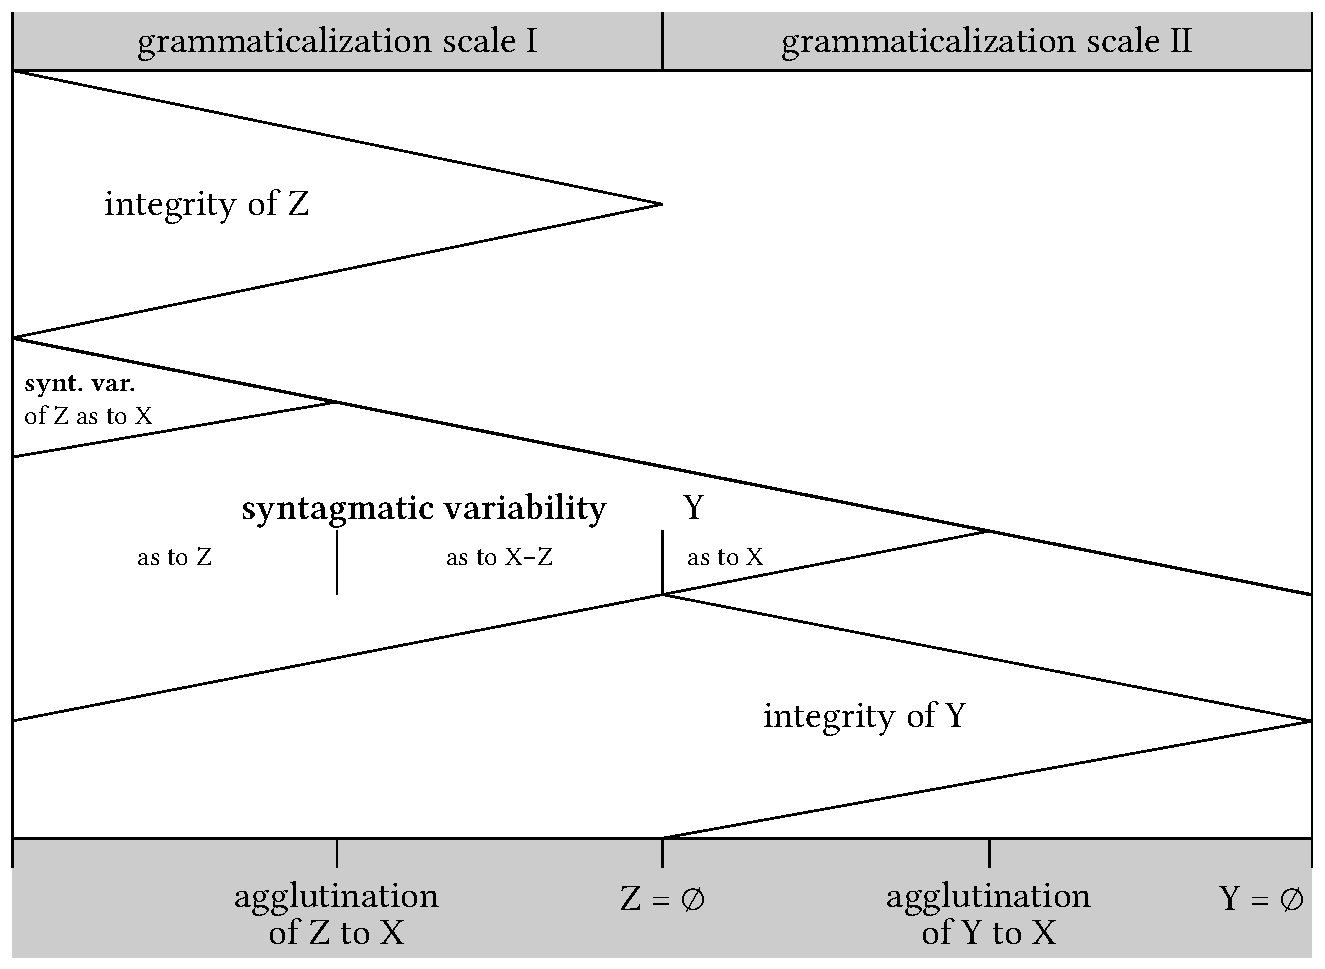
\includegraphics[width=\textwidth]{figures/12-reduction-to-zero.pdf}
	
\caption{Reduction to zero and fixation of word order}\label{F12}
\end{figure}
\figref{F12} sums up this discussion by displaying two things at once: first, the behavior of syntagmatic variability in both the primary and the secondary grammatical relations of Z while this is reduced to zero; and second, the phase-displacement of syntagmatic variability as against the other grammaticalization parameters, here represented by integrity.

\enlargethispage{1\baselineskip}
The picture is to be read as follows: One side of each of the two wedges symbolizing decrease in syntagmatic variability has been prolonged to the right, both to suggest that the notion continues to be applicable even after the agglutination stage, but that no further decrease occurs, and to illustrate how the carrier of the affix becomes the reference point for the secondary grammatical relation and exhibits syntagmatic variability with respect to a third term. We also see that at the point where Z becomes zero, word order between X and Y is already fairly fixed.

We may anticipate that the subsumption of word order in the framework of grammaticalization will lead to a new appraisal of the attempts to typologize languages according to their word-order patterns. This will be done in §7.2.

The last lesson that this discussion teaches concerns the level at which grammaticalization works. A view that concentrates on the historical fate of single words and morphemes is too atomistic. Grammaticalization reduces not only the integrity, but also the scope of a sign. This means that it shifts signs down the hierarchy of grammatical levels, and it does this simultaneously to a given sign and to the sign of which the former is a proper grammatical part. One cannot but agree with Givón's (\citeyear[94]{Givón1979}) proposal “to treat syntacticization and the rise of grammatical morphology as two mutually dependent parts of the same process.”

